\documentclass[dvipsnames, 11pt]{beamer}
\setbeamertemplate{footline}[frame number]
\setbeamertemplate{navigation symbols}{}
\setbeamercolor{footline}{fg=black}
\setbeamerfont{footline}{series=\bfseries}
\usepackage{appendixnumberbeamer}
\usepackage{tikz}
\usepackage[utf8]{inputenc}
\usepackage{booktabs}
\usepackage[mathscr]{euscript}
\usepackage{subcaption}
\usepackage{nicefrac}
\usetheme{Darmstadt}

%%% packages and libraries %%%
\usepackage{amsmath, amsthm, amssymb, amsfonts}
\usepackage{mathtools}
\usepackage{algorithm, algpseudocode}
\usepackage{xparse}

%%% custom stats commands %%%
\newcommand{\simiid}{\overset{\scriptscriptstyle{\textrm{i.i.d.}}}{\sim}}
\newcommand{\indep}{\mathrel{\perp\!\!\!\perp}}
\newcommand{\estm}[2][]{\widehat{#2}_{#1}} % estimator
\newcommand{\iter}[2]{{#1}^{(#2)}} % iteration of algorithm

%%% custom math commands %%%
% \newcommand{\tpose}[1]{#1^{\scriptstyle{\mathsf{T}}}} % transpose
% \newcommand{\ctpose}[1]{#1^{\scriptstyle{\mathsf{H}}}} % conjugate transpose
\newcommand{\floor}[1]{\lfloor{#1}\rfloor}
\newcommand{\ceil}[1]{\lceil{#1}\rceil}

\DeclareMathOperator*{\argmax}{arg\,max}
\DeclareMathOperator*{\argmin}{arg\,min}
\DeclareMathOperator{\sign}{sign}
\DeclareMathOperator{\sgn}{sgn}
\DeclareMathOperator{\rank}{rank}
\DeclareMathOperator{\spn}{span}
\DeclareMathOperator{\tr}{tr}
\DeclareMathOperator{\supp}{supp}

% probability of event (optional subscript, blank by default)
\NewDocumentCommand{\prob}{ s O{} m }{
    \IfBooleanTF{#1}
        {\bbP_{#2}(#3)}              % \prob*{} (no resizing)
        {\bbP_{#2}\!\left(#3\right)} % \prob (auto-sizing)
}

% expectation (optional subscript, blank by default)
\NewDocumentCommand{\expec}{ s O{} m }{
    \IfBooleanTF{#1}
        {\bbE_{#2}[#3]}              % \expec*{} (no resizing)
        {\bbE_{#2}\!\left[#3\right]} % \expec (auto-sizing)
}

% variance (optional subscript, blank by default)
\NewDocumentCommand{\var}{ s O{} m }{
    \IfBooleanTF{#1}
        {\operatorname{Var}_{#2}(#3)}              % \var*{} (no resizing)
        {\operatorname{Var}_{#2}\!\left(#3\right)} % \var (auto-sizing)
}

% covariance (optional subscript, blank by default)
\NewDocumentCommand{\covar}{ s O{} m m }{
    \IfBooleanTF{#1}
        {\operatorname{Cov}_{#2}(#3, #4)}              % \covar*{} (no resizing)
        {\operatorname{Cov}_{#2}\!\left(#3, #4\right)} % \covar (auto-sizing)
}

% correlation (optional subscript, blank by default)
\NewDocumentCommand{\corr}{ s O{} m m }{
    \IfBooleanTF{#1}
        {\operatorname{corr}_{#2}(#3, #4)}              % \corr*{} (no resizing)
        {\operatorname{corr}_{#2}\!\left(#3, #4\right)} % \corr (auto-sizing)
}

% bias (optional subscript, blank by default)
\NewDocumentCommand{\bias}{ s O{} m }{
    \IfBooleanTF{#1}
        {\operatorname{bias}_{#2}(#3)}              % \bias*{} (no resizing)
        {\operatorname{bias}_{#2}\!\left(#3\right)} % \bias (auto-sizing)
}

% MSE (optional subscript, blank by default)
\NewDocumentCommand{\MSE}{ s O{} m }{
    \IfBooleanTF{#1}
        {\operatorname{MSE}_{#2}(#3)}              % \MSE*{} (no resizing)
        {\operatorname{MSE}_{#2}\!\left(#3\right)} % \MSE (auto-sizing)
}

% "full" derivative 
\NewDocumentCommand{\dx}{ o }{
    \mathrm{d}
    \IfValueT{#1}{
        \IfBlankF{#1}{#1}
    }
}

% "full" derivative (fractional)
\NewDocumentCommand{\ddx}{ O{} m m }{
    \IfValueTF{#1}
        {\frac{\dx^{#1}#2}{\dx{#3^{#1}}}}
        {\frac{\dx{#2}}{\dx{#3}}}
}

% partial derivative
\NewDocumentCommand{\px}{ o }{
    \partial
    \IfValueT{#1}{
        \IfBlankF{#1}{#1}
    }
}

% partial derivative (fractional)
\NewDocumentCommand{\pdx}{ O{} m m }{
    \IfValueTF{#1}
        {\frac{\px^{#1}#2}{\px{#3^{#1}}}}
        {\frac{\px{#2}}{\px{#3}}}
}

% inner product (optional base, blank by default)
\NewDocumentCommand{\innerprod}{ s O{} m m }{
    \IfBooleanTF{#1}
        {\langle{#3},{#4}\rangle_{#2}}            % \innerprod*{} (no resizing)       
        {\left\langle{#3},{#4}\right\rangle_{#2}} % \innerprod{}  (auto-sizing)
}

% norm (optional base, blank by default)
\NewDocumentCommand{\norm}{ s O{} m }{
    \IfBooleanTF{#1}
        {\lVert{#3}\rVert_{#2}}            % \norm*{} (no resizing)
        {\left\lVert{#3}\right\rVert_{#2}} % \norm{}  (auto-sizing)
}

% absolute value
\NewDocumentCommand{\abs}{ s m }{
    \IfBooleanTF{#1}
        {\lvert{#2}\rvert}            % \abs*{} (no resizing)
        {\left\lvert{#2}\right\rvert} % \abs{}  (auto-sizing)
}
%%% packages and libraries %%%
\usepackage{mathtools}
\usepackage{amsmath, amsthm, amssymb, amsfonts}
\usepackage{bm}

%%% blackboard alphabet (uppercase) %%%
\newcommand{\bbA}{\mathbb{A}}
\newcommand{\bbB}{\mathbb{B}}
\newcommand{\bbC}{\mathbb{C}}
\newcommand{\bbD}{\mathbb{D}}
\newcommand{\bbE}{\mathbb{E}}
\newcommand{\bbF}{\mathbb{F}}
\newcommand{\bbG}{\mathbb{G}}
\newcommand{\bbH}{\mathbb{H}}
\newcommand{\bbI}{\mathbb{I}}
\newcommand{\bbJ}{\mathbb{J}}
\newcommand{\bbK}{\mathbb{K}}
\newcommand{\bbL}{\mathbb{L}}
\newcommand{\bbM}{\mathbb{M}}
\newcommand{\bbN}{\mathbb{N}}
\newcommand{\bbO}{\mathbb{O}}
\newcommand{\bbP}{\mathbb{P}}
\newcommand{\bbQ}{\mathbb{Q}}
\newcommand{\bbR}{\mathbb{R}}
\newcommand{\bbS}{\mathbb{S}}
\newcommand{\bbT}{\mathbb{T}}
\newcommand{\bbU}{\mathbb{U}}
\newcommand{\bbV}{\mathbb{V}}
\newcommand{\bbW}{\mathbb{W}}
\newcommand{\bbX}{\mathbb{X}}
\newcommand{\bbY}{\mathbb{Y}}
\newcommand{\bbZ}{\mathbb{Z}}

%%% calligraphic alphabet (uppercase) %%%
\newcommand{\calA}{\mathcal{A}}
\newcommand{\calB}{\mathcal{B}}
\newcommand{\calC}{\mathcal{C}}
\newcommand{\calD}{\mathcal{D}}
\newcommand{\calE}{\mathcal{E}}
\newcommand{\calF}{\mathcal{F}}
\newcommand{\calG}{\mathcal{G}}
\newcommand{\calH}{\mathcal{H}}
\newcommand{\calI}{\mathcal{I}}
\newcommand{\calJ}{\mathcal{J}}
\newcommand{\calK}{\mathcal{K}}
\newcommand{\calL}{\mathcal{L}}
\newcommand{\calM}{\mathcal{M}}
\newcommand{\calN}{\mathcal{N}}
\newcommand{\calO}{\mathcal{O}}
\newcommand{\calP}{\mathcal{P}}
\newcommand{\calQ}{\mathcal{Q}}
\newcommand{\calR}{\mathcal{R}}
\newcommand{\calS}{\mathcal{S}}
\newcommand{\calT}{\mathcal{T}}
\newcommand{\calU}{\mathcal{U}}
\newcommand{\calV}{\mathcal{V}}
\newcommand{\calW}{\mathcal{W}}
\newcommand{\calX}{\mathcal{X}}
\newcommand{\calY}{\mathcal{Y}}
\newcommand{\calZ}{\mathcal{Z}}

%%% standard alphabet (uppercase) %%%
\newcommand{\rmA}{\mathrm{A}}
\newcommand{\rmB}{\mathrm{B}}
\newcommand{\rmC}{\mathrm{C}}
\newcommand{\rmD}{\mathrm{D}}
\newcommand{\rmE}{\mathrm{E}}
\newcommand{\rmF}{\mathrm{F}}
\newcommand{\rmG}{\mathrm{G}}
\newcommand{\rmH}{\mathrm{H}}
\newcommand{\rmI}{\mathrm{I}}
\newcommand{\rmJ}{\mathrm{J}}
\newcommand{\rmK}{\mathrm{K}}
\newcommand{\rmL}{\mathrm{L}}
\newcommand{\rmM}{\mathrm{M}}
\newcommand{\rmN}{\mathrm{N}}
\newcommand{\rmO}{\mathrm{O}}
\newcommand{\rmP}{\mathrm{P}}
\newcommand{\rmQ}{\mathrm{Q}}
\newcommand{\rmR}{\mathrm{R}}
\newcommand{\rmS}{\mathrm{S}}
\newcommand{\rmT}{\mathrm{T}}
\newcommand{\rmU}{\mathrm{U}}
\newcommand{\rmV}{\mathrm{V}}
\newcommand{\rmW}{\mathrm{W}}
\newcommand{\rmX}{\mathrm{X}}
\newcommand{\rmY}{\mathrm{Y}}
\newcommand{\rmZ}{\mathrm{Z}}

%%% standard alphabet (lowercase) %%%
\newcommand{\rma}{\mathrm{a}}
\newcommand{\rmb}{\mathrm{b}}
\newcommand{\rmc}{\mathrm{c}}
\newcommand{\rmd}{\mathrm{d}}
\newcommand{\rme}{\mathrm{e}}
\newcommand{\rmf}{\mathrm{f}}
\newcommand{\rmg}{\mathrm{g}}
\newcommand{\rmh}{\mathrm{h}}
\newcommand{\rmi}{\mathrm{i}}
\newcommand{\rmj}{\mathrm{j}}
\newcommand{\rmk}{\mathrm{k}}
\newcommand{\rml}{\mathrm{l}}
\newcommand{\rmm}{\mathrm{m}}
\newcommand{\rmn}{\mathrm{n}}
\newcommand{\rmo}{\mathrm{o}}
\newcommand{\rmp}{\mathrm{p}}
\newcommand{\rmq}{\mathrm{q}}
\newcommand{\rmr}{\mathrm{r}}
\newcommand{\rms}{\mathrm{s}}
\newcommand{\rmt}{\mathrm{t}}
\newcommand{\rmu}{\mathrm{u}}
\newcommand{\rmv}{\mathrm{v}}
\newcommand{\rmw}{\mathrm{w}}
\newcommand{\rmx}{\mathrm{x}}
\newcommand{\rmy}{\mathrm{y}}
\newcommand{\rmz}{\mathrm{z}}

%%% boldface math alphabet (uppercase) %%%
\newcommand{\bfA}{\mathbf{A}}
\newcommand{\bfB}{\mathbf{B}}
\newcommand{\bfC}{\mathbf{C}}
\newcommand{\bfD}{\mathbf{D}}
\newcommand{\bfE}{\mathbf{E}}
\newcommand{\bfF}{\mathbf{F}}
\newcommand{\bfG}{\mathbf{G}}
\newcommand{\bfH}{\mathbf{H}}
\newcommand{\bfI}{\mathbf{I}}
\newcommand{\bfJ}{\mathbf{J}}
\newcommand{\bfK}{\mathbf{K}}
\newcommand{\bfL}{\mathbf{L}}
\newcommand{\bfM}{\mathbf{M}}
\newcommand{\bfN}{\mathbf{N}}
\newcommand{\bfO}{\mathbf{O}}
\newcommand{\bfP}{\mathbf{P}}
\newcommand{\bfQ}{\mathbf{Q}}
\newcommand{\bfR}{\mathbf{R}}
\newcommand{\bfS}{\mathbf{S}}
\newcommand{\bfT}{\mathbf{T}}
\newcommand{\bfU}{\mathbf{U}}
\newcommand{\bfV}{\mathbf{V}}
\newcommand{\bfW}{\mathbf{W}}
\newcommand{\bfX}{\mathbf{X}}
\newcommand{\bfY}{\mathbf{Y}}
\newcommand{\bfZ}{\mathbf{Z}}

%%% boldface math alphabet (lowercase) %%%
\newcommand{\bfa}{\mathbf{a}}
\newcommand{\bfb}{\mathbf{b}}
\newcommand{\bfc}{\mathbf{c}}
\newcommand{\bfd}{\mathbf{d}}
\newcommand{\bfe}{\mathbf{e}}
\newcommand{\bff}{\mathbf{f}}
\newcommand{\bfg}{\mathbf{g}}
\newcommand{\bfh}{\mathbf{h}}
\newcommand{\bfi}{\mathbf{i}}
\newcommand{\bfj}{\mathbf{j}}
\newcommand{\bfk}{\mathbf{k}}
\newcommand{\bfl}{\mathbf{l}}
\newcommand{\bfm}{\mathbf{m}}
\newcommand{\bfn}{\mathbf{n}}
\newcommand{\bfo}{\mathbf{o}}
\newcommand{\bfp}{\mathbf{p}}
\newcommand{\bfq}{\mathbf{q}}
\newcommand{\bfr}{\mathbf{r}}
\newcommand{\bfs}{\mathbf{s}}
\newcommand{\bft}{\mathbf{t}}
\newcommand{\bfu}{\mathbf{u}}
\newcommand{\bfv}{\mathbf{v}}
\newcommand{\bfw}{\mathbf{w}}
\newcommand{\bfx}{\mathbf{x}}
\newcommand{\bfy}{\mathbf{y}}
\newcommand{\bfz}{\mathbf{z}}

%%% bold italic alphabet (uppercase) %%%
\newcommand{\bmA}{\bm{A}}
\newcommand{\bmB}{\bm{B}}
\newcommand{\bmC}{\bm{C}}
\newcommand{\bmD}{\bm{D}}
\newcommand{\bmE}{\bm{E}}
\newcommand{\bmF}{\bm{F}}
\newcommand{\bmG}{\bm{G}}
\newcommand{\bmH}{\bm{H}}
\newcommand{\bmI}{\bm{I}}
\newcommand{\bmJ}{\bm{J}}
\newcommand{\bmK}{\bm{K}}
\newcommand{\bmL}{\bm{L}}
\newcommand{\bmM}{\bm{M}}
\newcommand{\bmN}{\bm{N}}
\newcommand{\bmO}{\bm{O}}
\newcommand{\bmP}{\bm{P}}
\newcommand{\bmQ}{\bm{Q}}
\newcommand{\bmR}{\bm{R}}
\newcommand{\bmS}{\bm{S}}
\newcommand{\bmT}{\bm{T}}
\newcommand{\bmU}{\bm{U}}
\newcommand{\bmV}{\bm{V}}
\newcommand{\bmW}{\bm{W}}
\newcommand{\bmX}{\bm{X}}
\newcommand{\bmY}{\bm{Y}}
\newcommand{\bmZ}{\bm{Z}}

%%% bold italic alphabet (lowercase) %%%
\newcommand{\bma}{\bm{a}}
\newcommand{\bmb}{\bm{b}}
\newcommand{\bmc}{\bm{c}}
\newcommand{\bmd}{\bm{d}}
\newcommand{\bme}{\bm{e}}
\newcommand{\bmf}{\bm{f}}
\newcommand{\bmg}{\bm{g}}
\newcommand{\bmh}{\bm{h}}
\newcommand{\bmi}{\bm{i}}
\newcommand{\bmj}{\bm{j}}
\newcommand{\bmk}{\bm{k}}
\newcommand{\bml}{\bm{l}}
\newcommand{\bmm}{\bm{m}}
\newcommand{\bmn}{\bm{n}}
\newcommand{\bmo}{\bm{o}}
\newcommand{\bmp}{\bm{p}}
\newcommand{\bmq}{\bm{q}}
\newcommand{\bmr}{\bm{r}}
\newcommand{\bms}{\bm{s}}
\newcommand{\bmt}{\bm{t}}
\newcommand{\bmu}{\bm{u}}
\newcommand{\bmv}{\bm{v}}
\newcommand{\bmw}{\bm{w}}
\newcommand{\bmx}{\bm{x}}
\newcommand{\bmy}{\bm{y}}
\newcommand{\bmz}{\bm{z}}

%%% sans-serif alphabet (uppercase) %%%
\newcommand{\sfA}{\mathsf{A}}
\newcommand{\sfB}{\mathsf{B}}
\newcommand{\sfC}{\mathsf{C}}
\newcommand{\sfD}{\mathsf{D}}
\newcommand{\sfE}{\mathsf{E}}
\newcommand{\sfF}{\mathsf{F}}
\newcommand{\sfG}{\mathsf{G}}
\newcommand{\sfH}{\mathsf{H}}
\newcommand{\sfI}{\mathsf{I}}
\newcommand{\sfJ}{\mathsf{J}}
\newcommand{\sfK}{\mathsf{K}}
\newcommand{\sfL}{\mathsf{L}}
\newcommand{\sfM}{\mathsf{M}}
\newcommand{\sfN}{\mathsf{N}}
\newcommand{\sfO}{\mathsf{O}}
\newcommand{\sfP}{\mathsf{P}}
\newcommand{\sfQ}{\mathsf{Q}}
\newcommand{\sfR}{\mathsf{R}}
\newcommand{\sfS}{\mathsf{S}}
\newcommand{\sfT}{\mathsf{T}}
\newcommand{\sfU}{\mathsf{U}}
\newcommand{\sfV}{\mathsf{V}}
\newcommand{\sfW}{\mathsf{W}}
\newcommand{\sfX}{\mathsf{X}}
\newcommand{\sfY}{\mathsf{Y}}
\newcommand{\sfZ}{\mathsf{Z}}

%%% sans-serif alphabet (lowercase) %%%
\newcommand{\sfa}{\mathsf{a}}
\newcommand{\sfb}{\mathsf{b}}
\newcommand{\sfc}{\mathsf{c}}
\newcommand{\sfd}{\mathsf{d}}
\newcommand{\sfe}{\mathsf{e}}
\newcommand{\sff}{\mathsf{f}}
\newcommand{\sfg}{\mathsf{g}}
\newcommand{\sfh}{\mathsf{h}}
\newcommand{\sfi}{\mathsf{i}}
\newcommand{\sfj}{\mathsf{j}}
\newcommand{\sfk}{\mathsf{k}}
\newcommand{\sfl}{\mathsf{l}}
\newcommand{\sfm}{\mathsf{m}}
\newcommand{\sfn}{\mathsf{n}}
\newcommand{\sfo}{\mathsf{o}}
\newcommand{\sfp}{\mathsf{p}}
\newcommand{\sfq}{\mathsf{q}}
\newcommand{\sfr}{\mathsf{r}}
\newcommand{\sfs}{\mathsf{s}}
\newcommand{\sft}{\mathsf{t}}
\newcommand{\sfu}{\mathsf{u}}
\newcommand{\sfv}{\mathsf{v}}
\newcommand{\sfw}{\mathsf{w}}
\newcommand{\sfx}{\mathsf{x}}
\newcommand{\sfy}{\mathsf{y}}
\newcommand{\sfz}{\mathsf{z}}

%%% bold italic sans-serif alphabet (uppercase) %%%
% \newcommand{\bsfA}{\mathbfsf{A}}
% \newcommand{\bsfB}{\mathbfsf{B}}
% \newcommand{\bsfC}{\mathbfsf{C}}
% \newcommand{\bsfD}{\mathbfsf{D}}
% \newcommand{\bsfE}{\mathbfsf{E}}
% \newcommand{\bsfF}{\mathbfsf{F}}
% \newcommand{\bsfG}{\mathbfsf{G}}
% \newcommand{\bsfH}{\mathbfsf{H}}
% \newcommand{\bsfI}{\mathbfsf{I}}
% \newcommand{\bsfJ}{\mathbfsf{J}}
% \newcommand{\bsfK}{\mathbfsf{K}}
% \newcommand{\bsfL}{\mathbfsf{L}}
% \newcommand{\bsfM}{\mathbfsf{M}}
% \newcommand{\bsfN}{\mathbfsf{N}}
% \newcommand{\bsfO}{\mathbfsf{O}}
% \newcommand{\bsfP}{\mathbfsf{P}}
% \newcommand{\bsfQ}{\mathbfsf{Q}}
% \newcommand{\bsfR}{\mathbfsf{R}}
% \newcommand{\bsfS}{\mathbfsf{S}}
% \newcommand{\bsfT}{\mathbfsf{T}}
% \newcommand{\bsfU}{\mathbfsf{U}}
% \newcommand{\bsfV}{\mathbfsf{V}}
% \newcommand{\bsfW}{\mathbfsf{W}}
% \newcommand{\bsfX}{\mathbfsf{X}}
% \newcommand{\bsfY}{\mathbfsf{Y}}
% \newcommand{\bsfZ}{\mathbfsf{Z}}

%%% bold italic sans-serif alphabet (lowercase) %%%
% \newcommand{\bsfa}{\mathbfsf{a}}
% \newcommand{\bsfb}{\mathbfsf{b}}
% \newcommand{\bsfc}{\mathbfsf{c}}
% \newcommand{\bsfd}{\mathbfsf{d}}
% \newcommand{\bsfe}{\mathbfsf{e}}
% \newcommand{\bsff}{\mathbfsf{f}}
% \newcommand{\bsfg}{\mathbfsf{g}}
% \newcommand{\bsfh}{\mathbfsf{h}}
% \newcommand{\bsfi}{\mathbfsf{i}}
% \newcommand{\bsfj}{\mathbfsf{j}}
% \newcommand{\bsfk}{\mathbfsf{k}}
% \newcommand{\bsfl}{\mathbfsf{l}}
% \newcommand{\bsfm}{\mathbfsf{m}}
% \newcommand{\bsfn}{\mathbfsf{n}}
% \newcommand{\bsfo}{\mathbfsf{o}}
% \newcommand{\bsfp}{\mathbfsf{p}}
% \newcommand{\bsfq}{\mathbfsf{q}}
% \newcommand{\bsfr}{\mathbfsf{r}}
% \newcommand{\bsfs}{\mathbfsf{s}}
% \newcommand{\bsft}{\mathbfsf{t}}
% \newcommand{\bsfu}{\mathbfsf{u}}
% \newcommand{\bsfv}{\mathbfsf{v}}
% \newcommand{\bsfw}{\mathbfsf{w}}
% \newcommand{\bsfx}{\mathbfsf{x}}
% \newcommand{\bsfy}{\mathbfsf{y}}
% \newcommand{\bsfz}{\mathbfsf{z}}

%%% miscellaneous useful symbol commands %%%
\newcommand{\bfbeta}{\bm{\beta}}
\newcommand{\bfepsilon}{\bm{\epsilon}}
\newcommand{\bfmu}{\bm{\mu}}
\newcommand{\bftheta}{\bm{\theta}}
\newcommand{\bfSigma}{\bm{\Sigma}}

\newcommand{\sfTsmall}{\scriptstyle{\mathsf{T}}}
\newcommand{\sfHsmall}{\scriptstyle{\mathsf{H}}}

\usepackage{natbib}
\bibliographystyle{apalike}
\usepackage{graphicx}
% \graphicspath{{../Code/results/full/} {./images/}}
\graphicspath{{./images/}}

\newcommand{\calGP}{\mathcal{GP}}
\DeclareMathOperator{\vect}{vec}

\setbeamertemplate{caption}[numbered]
\setbeamertemplate{theorems}[numbered]
\newtheorem{assumption}{Assumption}

\newenvironment{theoremblock}[1]
{
    \setbeamercolor{block title}{bg=green!60!black, fg=white}
    \setbeamercolor{block body}{bg=green!5, fg=black}
    \begin{theorem}[#1]
}
{
    \end{theorem}
}
\newenvironment{definitionblock}[1]
{
    \setbeamercolor{block title}{bg=green!60!black, fg=white}
    \setbeamercolor{block body}{bg=green!5, fg=black}
    \begin{definition}[#1]
}
{
    \end{definition}
}
\newenvironment{assumptionblock}[1]
{
    \setbeamercolor{block title}{bg=red!75!black, fg=white}
    \setbeamercolor{block body}{bg=red!5, fg=black}
    \begin{assumption}[#1]
}
{
    \end{assumption}
}

\title{Computationally Efficient Predictions for\\Multi-Output Spatiotemporal Dynamical Systems}
\author{Joey Hotz}
% \institute{
%     Department of Statistical Sciences, University of Toronto\\[6pt]
%     \small Supervisor: Dr.\ Meredith Franklin\\
%     Examiners: Dr.\ Ricardo Baptista \& Dr.\ Joshua Speagle
% }
\institute{
    Department of Statistical Sciences, University of Toronto\\
}
\date{\today}

\begin{document}

\begin{frame}
    \titlepage
\end{frame}

\begin{frame}{Outline}
    \tableofcontents
\end{frame}

\section{Introduction}

\begin{frame}{Motivation}
    \begin{itemize}
        \item 
        Gaussian processes (GPs) are frequently used in modelling unknown functions based on correlated and noisy observations \citep{GPML-Book-2006}. 
        \item 
        GP regression (\emph{kriging}) yields tractable closed-form solutions. Kriging is widely employed in fields such as geostatistics, control systems, and ecology to learn from spatiotemporal observations.
        \item 
        \textbf{Major Drawback:} Performing exact inference on $N$ observations requires $\calO(N^3)$ operations.
        \begin{itemize}
            \item With repeated measurements, this cost grows cubically in both the number of locations \emph{and} measurements per location.
            \item Proposed remedies for the cubic scaling cost must trade exactness for computational efficiency.
        \end{itemize}
    \end{itemize}
\end{frame}

\begin{frame}{Project Overview}
    \begin{itemize}
        \item 
        \citet{Todescato-Efficient-2020} propose an algorithm which uses GP regression in tandem with the \textbf{Kalman filter} to efficiently estimate the state of a spatiotemporal dynamical system.
        \item 
        Under certain assumptions on the covariance structure, their algorithm accounts for spatial \emph{and} temporal dynamics.
        \item 
        \textbf{Problem:} The algorithm proposed by \citeauthor{Todescato-Efficient-2020} only considers scalar (univariate) responses.
        \item
        \textbf{Extension:} This work adapts the algorithm of \citeauthor{Todescato-Efficient-2020} for multivariate response vectors, including cases where responses are correlated.
    \end{itemize}
\end{frame}

\section{Background}

\begin{frame}{Univariate Gaussian Processes}
    \begin{definitionblock}{Gaussian Process}
    \label{def:GP}
        $f: \calX \to \bbR$ is a GP on $\calX$ if for all finite $\{\bfx_{1}, \dots, \bfx_{N}\} \subseteq \calX$, the random vector $\big(f(\bfx_{1}), \dots, f(\bfx_{N})\big)^{\sfTsmall}$ follows a multivariate Gaussian.
    \end{definitionblock}
    \begin{itemize}
        \item 
        A GP on $\calX$ is \emph{uniquely} determined by its mean $m(\bfx) = \expec{f(\bfx)}$ and kernel $k(\bfx, \bfx') = \covar{f(\bfx)}{f(\bfx')}$. 
        \item 
        For  noisy observations $y_{i} = f(\bfx_{i}) + \varepsilon_{i}$ with $\varepsilon_{i} \simiid \calN(0, \sigma^2)$:
        {\small
        \begin{equation*}
            \bfy \sim \calN\big(m(\bfX), k(\bfX, \bfX) + \sigma^{2}\bfI_{N}\big)
        \end{equation*}
        }
        \item 
        The posterior predictive distribution remains a GP:
        {\small
        \begin{align*}
            m_{\textrm{post}}(\bfx) &= m(\bfx) + k(\bfx, \bfX)\big[k(\bfX, \bfX) + \sigma^{2}\bfI_{N}\big]^{-1}\big(\bfy - m(\bfX)\big)\\
            k_{\textrm{post}}(\bfx, \bfx') &= k(\bfx, \bfx') - k(\bfx, \bfX)\big[k(\bfX, \bfX) + \sigma^{2}\bfI_{N}\big]^{-1}k(\bfX, \bfx')
        \end{align*}
        }
    \end{itemize}
\end{frame}

\begin{frame}{Linear Gaussian State Space Model}
    \begin{definitionblock}{Linear Gaussian State Space Model}
        \vspace{-1em}
        {\small
        \begin{align*}
            \textbf{Initial state:} \quad & \bfs(0) \sim \calN\big(\bfm(0), \bfSigma(0)\big)\\
            \textbf{Dynamic model:} \quad & \bfs(j+1) = \bfA(j)\bfs(j) + \bfw(j), && \bfw(j) \sim \calN\big(\mathbf{0}, \bfQ(j)\big)\\
            \textbf{Observation model:} \quad & \bfy(j) = \bfC(j)\bfs(j) + \bfv(j), && \bfv(j) \sim \calN\big(\mathbf{0}, \bfR(j)\big)
        \end{align*}
        }
    \end{definitionblock}
    \begin{itemize}
        \item
        The noise terms $\bfv(j)$ and $\bfw(j)$ in the model are mutually independent. The state transition matrices $\bfA(j)$ and $\bfC(j)$ are all known, as are the noise covariances $\bfQ(j)$ and $\bfR(j)$.
        \item 
        Every state $\bfs(j) \in \bbR^{d_{s}}$ and observation $\bfy \in \bbR^{d_{y}}$ is a Gaussian random vector with tractable mean and covariance parameters.
    \end{itemize}
\end{frame}

\begin{frame}{Linear Gaussian State Space Model}
    \begin{figure}[htbp]
        \centering
        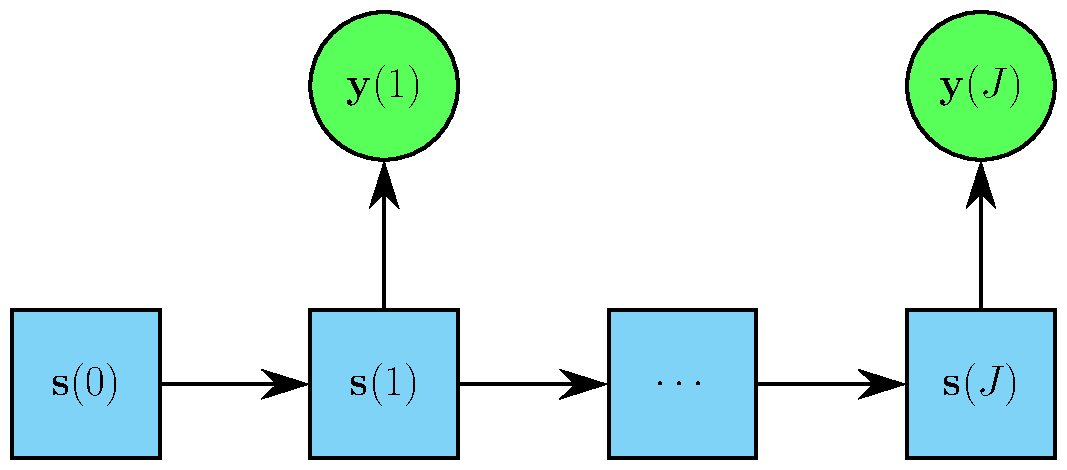
\includegraphics[width=0.9\textwidth]{LGSSM-diagram.pdf}

        \caption{A diagram of the state transitions and observations in a linear Gaussian state space model}
    \end{figure}
\end{frame}

\begin{frame}{Kalman Filtering}
    \begin{itemize}
        \item 
        The Kalman filter \citep{Kalman-Filter-1960} recursively estimates the latent states of a linear dynamical system (LGSSM) based on noisy indirect measurements.
        \item
        Each iteration of the Kalman filtering algorithm alternates between a \emph{prediction} and an \emph{update} step.
        \item
        \textbf{Computational Cost:} The per-iteration cost is $\calO(d_{s}^{3} + d_{y}^{3})$, and total cost is $\calO\big(J(d_{s}^{3} + d_{y}^{3})\big)$ \citep{Kalman-Complexity-2019}. This cost is \textbf{linear} is the number of observation times $J$.
    \end{itemize}
\end{frame}

\section{Prior Research}

\begin{frame}{Problem Setting \citep{Todescato-Efficient-2020}}
    \begin{itemize}
        \item 
        We have a compact state space $\calX \subset \bbR^{P}$, and finite set of observable locations $\calI = \{x_{1}, \dots, x_{M}\} \subseteq \calX$. 
        \item 
        Unknown function $f: \calX \times \bbR^{+} \to \bbR$, with $f \sim \calGP(0, K)$. Observations at instances $t_{0} < t_{1} < \cdots < t_{J}$, described by
        \begin{equation*}
            y_{i}(t_{j}) = f(x_{i}, t_{j}) + v_{i}(t_{j}), \quad v_{i}(t_{j}) \simiid \calN(0, \sigma^{2})
        \end{equation*}
        % \item
        % \textbf{Goal:} Estimate $f(x, t)$ at \emph{any} $x \in \calX$ and $t \in \bbR^{+}$.
        \item
        Observed subset $\calM_{j} \subseteq \calI$ ($M_{j} := \abs{\calM_{j}}$) may vary.
    \end{itemize}   

    \uncover<2->{    
    % \begin{assumption}[Kernel Separability]
    %     $K((x, t), (x', t')) = K_{s}(x, x')\,\gamma(\tau)$, where $\tau := \abs{t - t'}$.
    % \end{assumption}
    \begin{assumptionblock}{Kernel Separability}
        $K((x, t), (x', t')) = K_{s}(x, x')\,\gamma(\tau)$, where $\tau := \abs{t - t'}$.
    \end{assumptionblock}
    }

    \uncover<3->{
    % \begin{assumption}[Rational Power Spectrum]
    %     The power spectral density $S(\omega)$ of $\gamma(\tau)$ is a rational function of order $2r$.
    % \end{assumption}
    \begin{assumptionblock}{Rational Power Spectrum}
        The power spectral density $S(\omega)$ of $\gamma(\tau)$ is a rational function of order $2r$.
    \end{assumptionblock}
    }
\end{frame}

\begin{frame}{Dynamic Representer Theorem}
    \begin{theoremblock}{Dynamic Representer Theorem}
        Under Assumptions 1 and 2, for any $x \in \calX$ and $t \ge t_{J}$, the Kalman-enhanced regression algorithm of \citeauthor{Todescato-Efficient-2020} yields a minimum-variance estimator $\widehat{f}(x, t)$ of $f(x, t)$. 
    \end{theoremblock}
    \begin{itemize}
        \item 
        \textbf{Key Lemma:} $f(x, t) \indep \bff(t') \mid \bff(t)$ for $t' \ne t$.
        \item
        The filtered output $\widehat{\bff}(t)$ from the Kalman-enhanced algorithm serves as a posterior GP over $\calI$ at time $t$. The posterior $\widehat{\bff}(t)$ can be used to compute a minimum-variance estimator of $f(x, t)$ at any $x \in \calX$.
        \item 
        Cost per update is $\calO(rMM_{j} + rM_{j}^{3})$ when the matrix $\overline{K}_{s}(\calI, \calI)^{-1}$ is precomputed. 
    \end{itemize}
\end{frame}

\section{Extension}

\begin{frame}{Multi-Output Gaussian Processes}
    \begin{definitionblock}{Multi-Output Gaussian Process}
    \label{def:MOGP}
        $\bff = (f_{1}, \dots, f_{D})^{\sfTsmall}: \calX \to \bbR^{D}$ is an MOGP on $\calX$ if for all finite $\{\bfx_{1}, \dots, \bfx_{N}\} \subseteq \calX$, the $ND$ values $f_{d}(\bfx_{i})$ are jointly Gaussian.
    \end{definitionblock}
    \begin{itemize}
        \item 
        MOGPs model \emph{auto-correlations} within a response vector and \emph{cross-correlations} between responses \citep{Alvarez-Vector-Kernels-2012}.
        \item 
        The Gram matrix $\bfK(\bfX, \bfX) \in \bbR^{ND \times ND}$ is built from $N^{2}$ $D \times D$ covariance sub-matrices. 
        \item
        In general, the computational cost of MOGP inference on $N$ $D$-dimensional responses is $\calO(N^{3}D^{3})$.
    \end{itemize}
\end{frame}

\begin{frame}{Structured MOGP Kernels}
    \begin{itemize}
        \item 
        \textbf{Independent:} $f_{d} \sim \calGP(m_{d}, k_{d})$ are independent univariate GPs. The Gram matrix $\bfK(\bfX, \bfX)$ is block-diagonal.
        \item
        \textbf{Linear Model of Coregionalization (LMC):} Output functions $\{f_{d}\}_{d=1}^{D}$ are linear combinations of independent latent GPs $u_{q}^{i} \sim \calGP(0, k^{(q)})$, with 
        \vspace*{-1em}
        {\small
        \begin{align*}
            f_{d}(\bfx) &= m_{d}(\bfx) + \sum_{q=1}^{Q}\sum_{i=1}^{R_{q}}\alpha_{d,q}^{i}u_{q}^{i}(\bfx)\\[-0.5em]
            \bfK(\bfX, \bfX) &= \sum_{q=1}^{Q}k^{(q)}(\bfX, \bfX) \otimes \bfB^{(q)}
        \end{align*}
        }
        \item 
        \textbf{Intrinsic Coregionalization Model (ICM):} A special case of the LMC kernel with $Q = 1$. Yields a Gram matrix of the form $\bfK(\bfX, \bfX) = k(\bfX, \bfX) \otimes \bfB$.
    \end{itemize}
\end{frame}

\begin{frame}{Multi-Output Setting}
    \begin{itemize}
        \item
        Unknown function $f: \calX \times \bbR^{+} \to \bbR^{D}$, with $f \sim \calGP(0, \bfK)$.
        \item 
        Observe data at instances $t_{0} < t_{1} < \cdots < t_{J}$, described by
        \begin{equation*}
            \bfy_{i}(t_{j}) = \bff(\bfx_{i}, t_{j}) + \bfv_{i}(t_{j}), \quad \bfv_{i}(t_{j}) \simiid \calN(0, \bfV)
        \end{equation*}
        \item
        \textbf{Relaxed Separability Assumption:} The MOGP kernel function $\bfK$ is a sum of $Q$ time-separable kernels.
        \item
        The setting considered by \citeauthor{Todescato-Efficient-2020} is the special case where $Q = 1, D = 1$. 
    \end{itemize}
    \uncover<2->{
    \begin{assumptionblock}{All-or-Nothing Missingness}
        For any location $\bfx_{i}$ and time $t_{j}$, the $D$ entries of $\bfy_{i}(t_{j}) \in \bbR^{D}$ are either all available, or all missing.
    \end{assumptionblock}
    }
\end{frame}

\begin{frame}{Simulation Kernels}
    For our simulation study, we focus on four MOGP kernel settings:
    {\small
    \begin{align*}
        \textbf{Independent:} &\quad \exp(-\abs{t - t'})K_{\textrm{RBF}}(x, x')\sigma^{2}_{d}\mathbf{1}_{\{d = d'\}}\\
        \textbf{ICM:} &\quad \exp(-\abs{t - t'})K_{\textrm{RBF}}(x, x')\bfB(d, d')\\
        \textbf{LMC:} &\quad \exp(-\abs{t - t'})\sum_{q=1}^{3}C_{7/2 - q}(x, x')\bfB^{(q)}(d, d')\\
        \textbf{Temporal LMC:} &\quad \sum_{q=1}^{3}\exp\!\Big(\!-\frac{\abs{t - t'}}{q}\Big)C_{7/2 - q}(x, x')\bfB^{(q)}(d, d')
    \end{align*}
    }
    $K_{\textrm{RBF}}$ represents the RBF kernel function, and $C_{\nu}$ is the Mat{\'e}rn covariance with parameter $\nu$. 
\end{frame}

\begin{frame}{Simulation Details}
    \begin{itemize}
        \item 
        Simulated observations generated from a zero-mean MOGP at 150 evenly-spaced locations on a 1-D grid, observed at 21 times $t \in \{0, \nicefrac{1}{2}, \dots, 10\}$.
        \item
        80\% of locations are observed, 20\% held out for prediction.
        \item
        A fixed proportion $\rho$ of observations are randomly deleted.
        \item
        Full-factorial design, with 20 simulations per combination:
        \begin{itemize}
            \item MOGP Kernels: Independent, ICM, LMC, Temporal LMC
            \item Output dimension $D \in \{1, 2, 3, 5\}$
            \item Missingness proportion $\rho \in \{0, 0.2, 0.5\}$
        \end{itemize}
        \item
        Implemented in Python 3.12 \citep{python-3-12-5} using \texttt{GPyTorch} \citep{GPyTorch-Library-2018}, based on MATLAB code from \citet{Carron-ML-Kalman-2016} and \citet{Todescato-Efficient-2020}. 
    \end{itemize}
\end{frame}

\section{Results}
\begin{frame}{Results: RMSE}
    \begin{figure}[htbp]
        \centering
        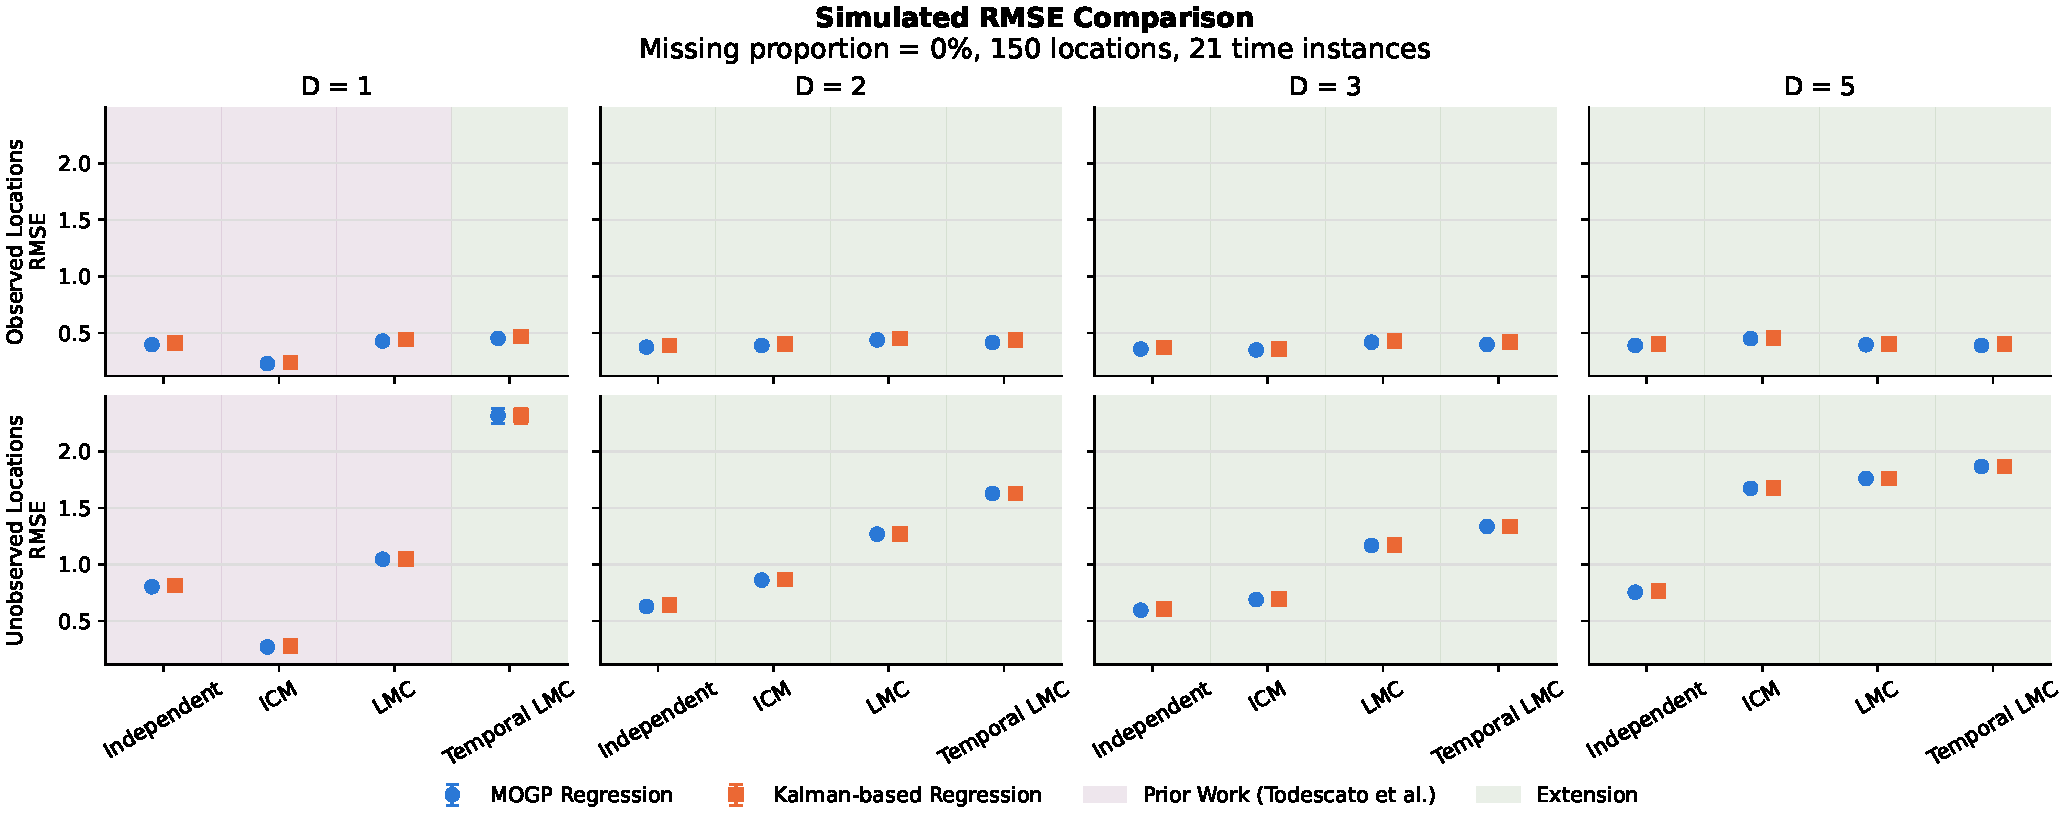
\includegraphics[height=0.35\textheight]{shaded_plots/rmse_missing_frac=0.0.pdf}\\[1em]
        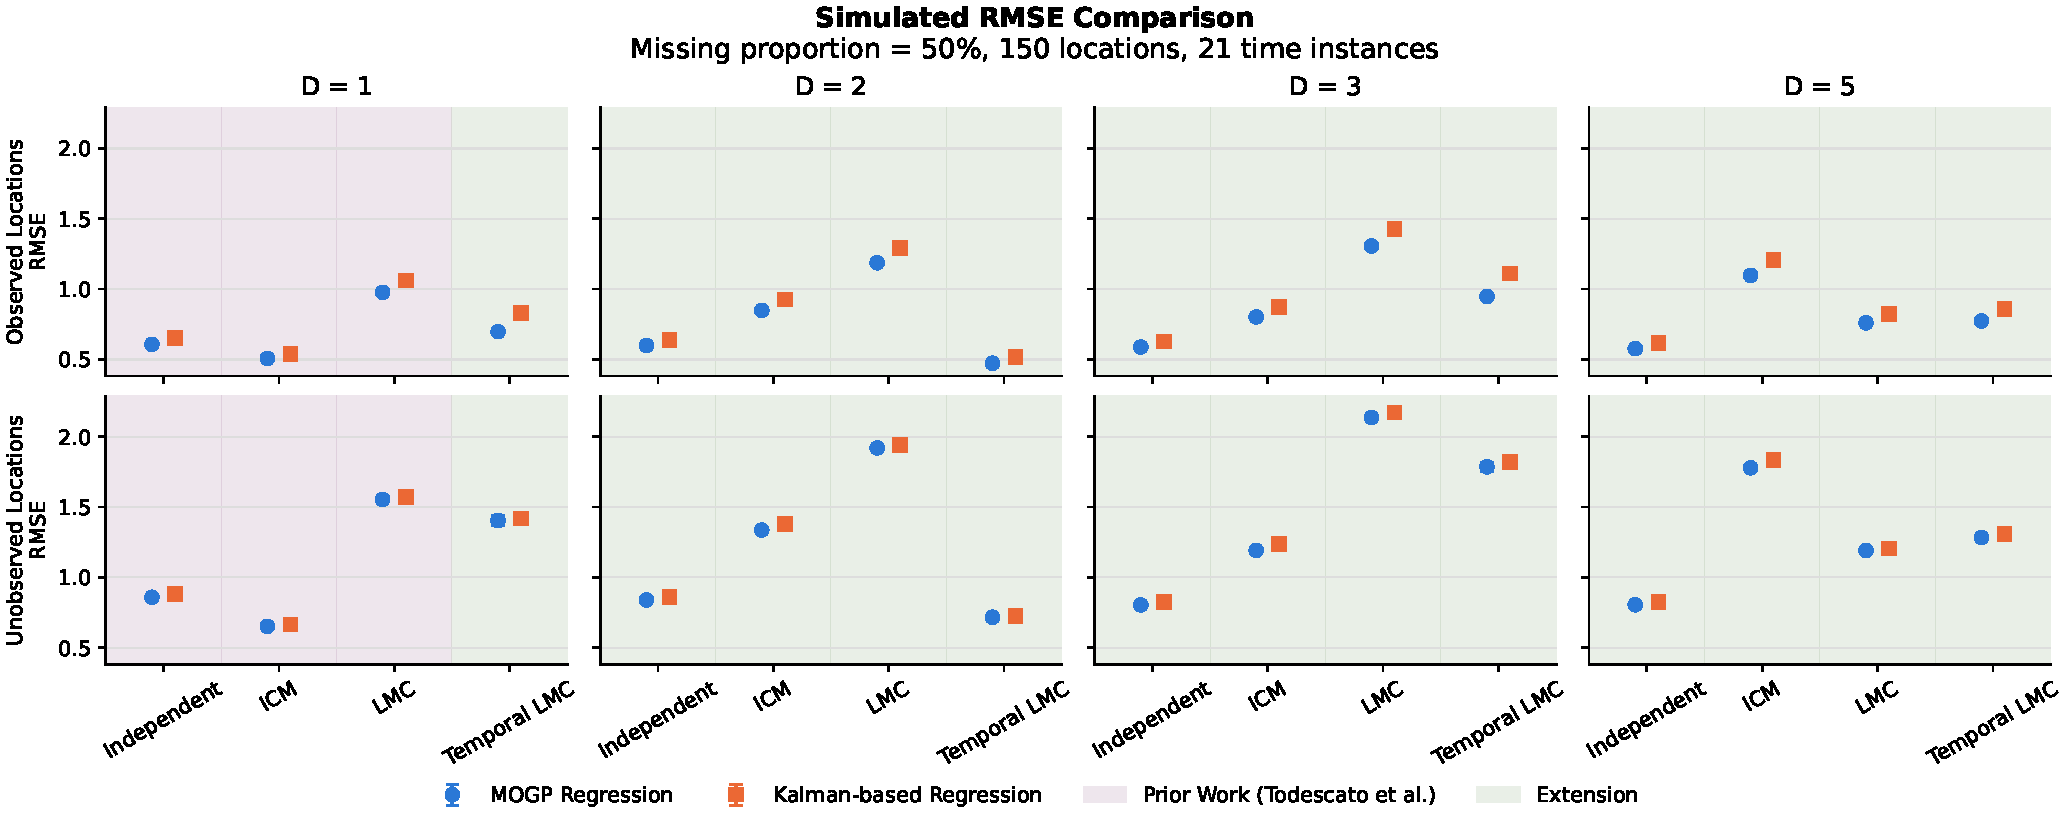
\includegraphics[height=0.35\textheight]{shaded_plots/rmse_missing_frac=0.5.pdf}

        \caption{{\small Plots of RMSE for $\rho = 0\%$ (top) and $\rho = 50\%$ (bottom)}}
    \end{figure}
\end{frame}

\begin{frame}{Results: Wall Clock Time}
    \begin{figure}[htbp]
        \centering
        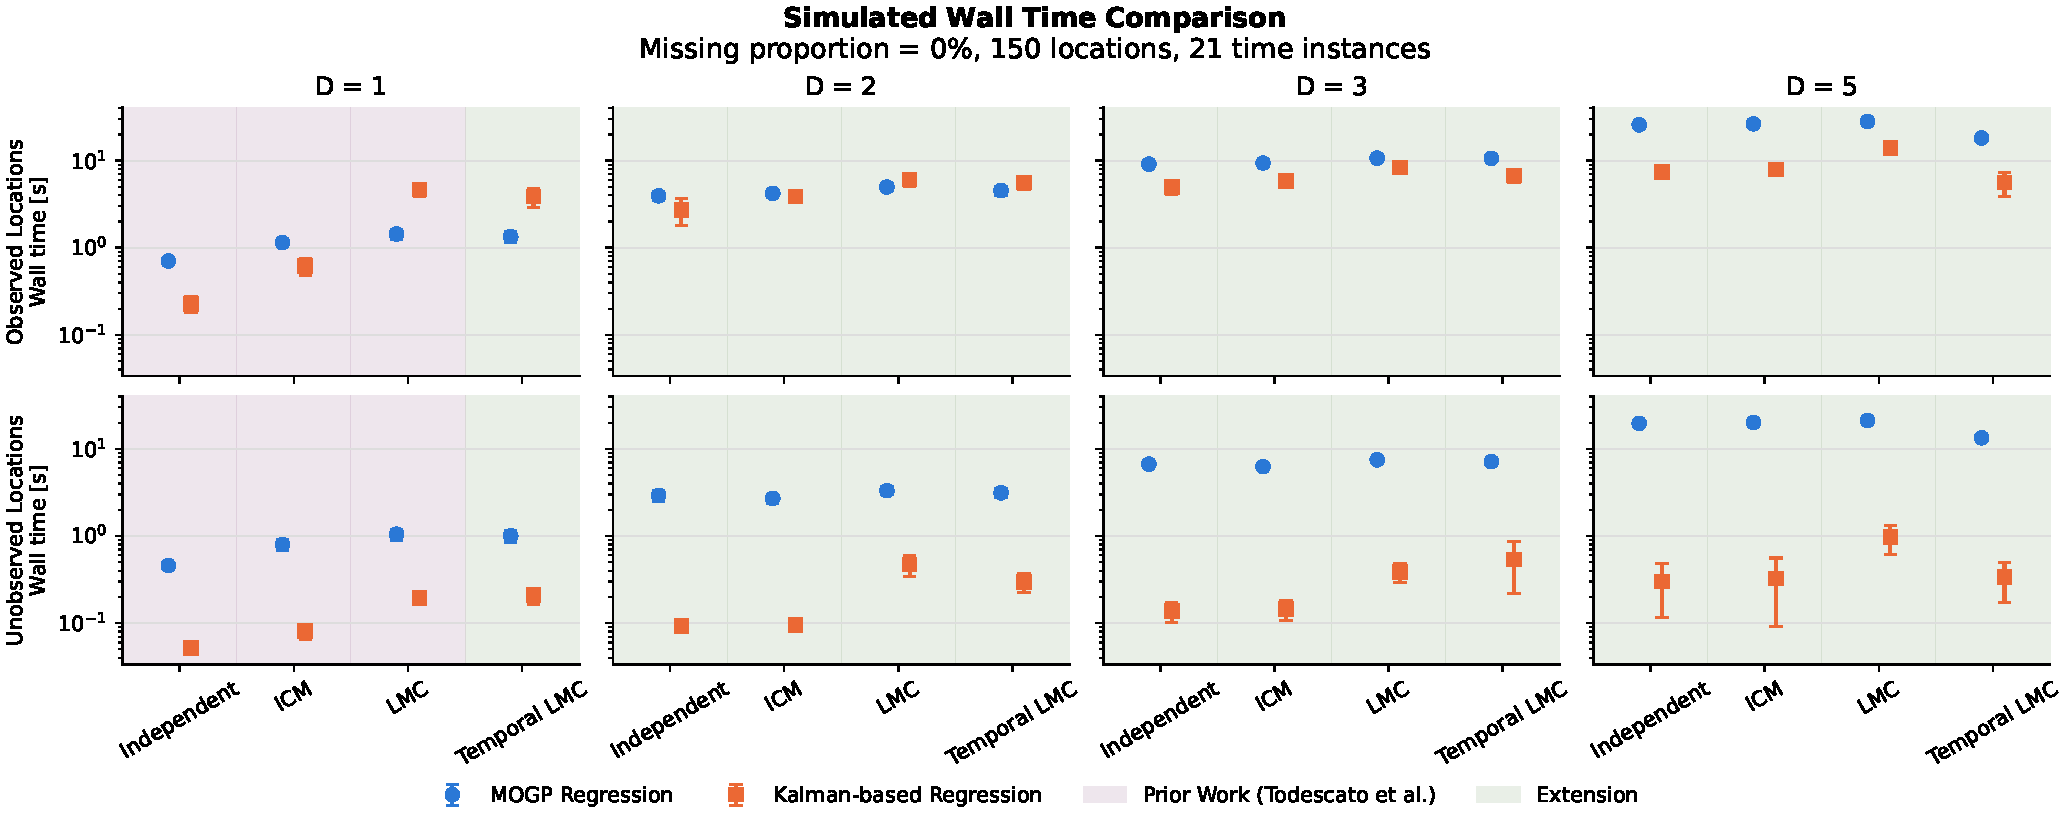
\includegraphics[height=0.35\textheight]{shaded_plots/wall_time_missing_frac=0.0.pdf}\\[1em]
        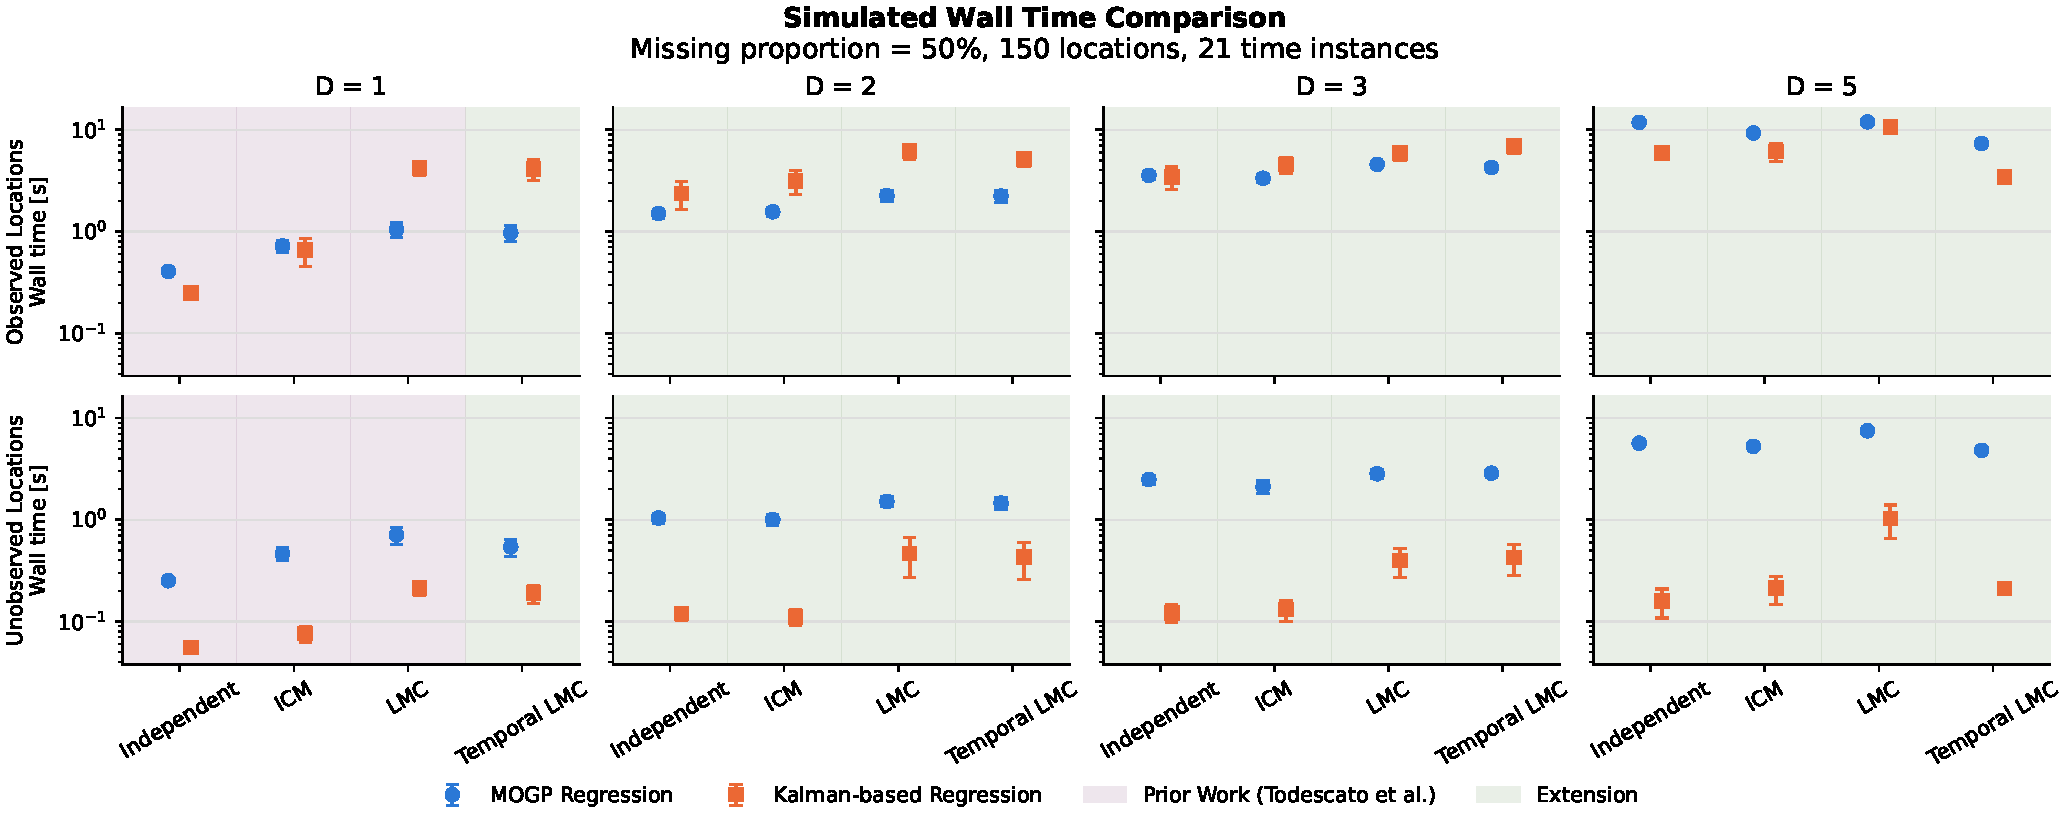
\includegraphics[height=0.35\textheight]{shaded_plots/wall_time_missing_frac=0.5.pdf}

        \caption{{\small Plots of elapsed wall clock time for $\rho = 0\%$ (top) and $\rho = 50\%$ (bottom)}}
    \end{figure}
\end{frame}

% \begin{frame}{Results: Coverage}
%     \begin{figure}[htbp]
%         \centering
%         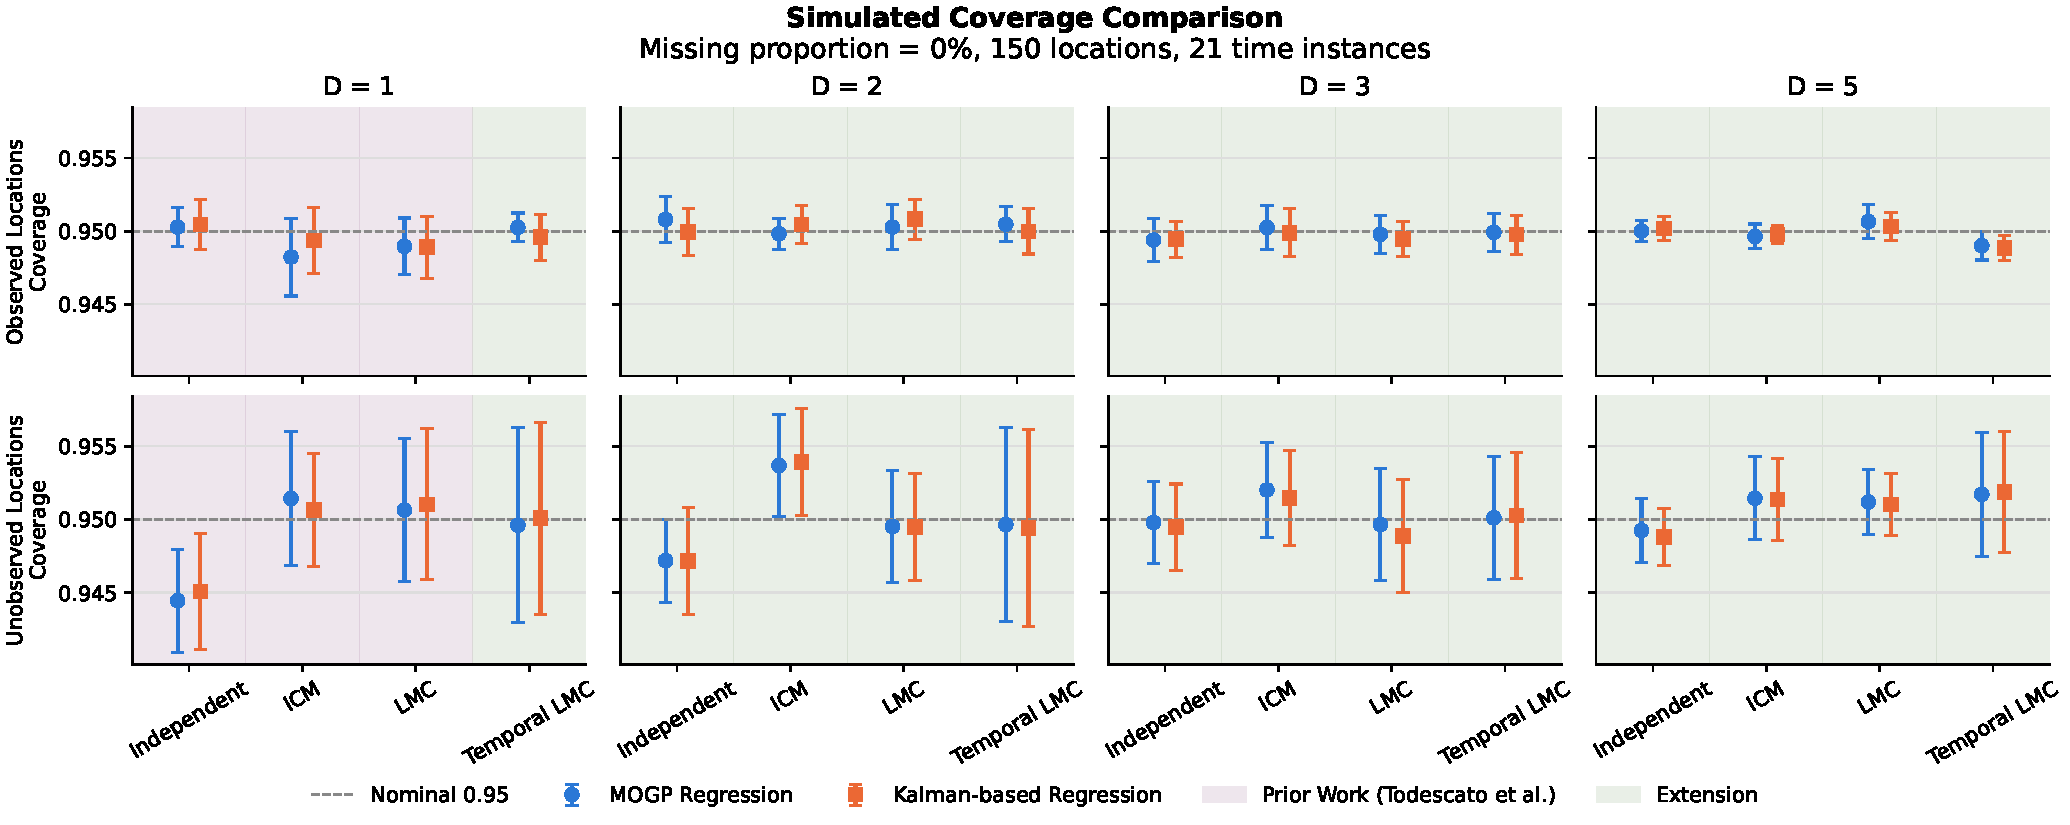
\includegraphics[height=0.35\textheight]{shaded_plots/coverage_missing_frac=0.0.pdf}\\[1em]
%         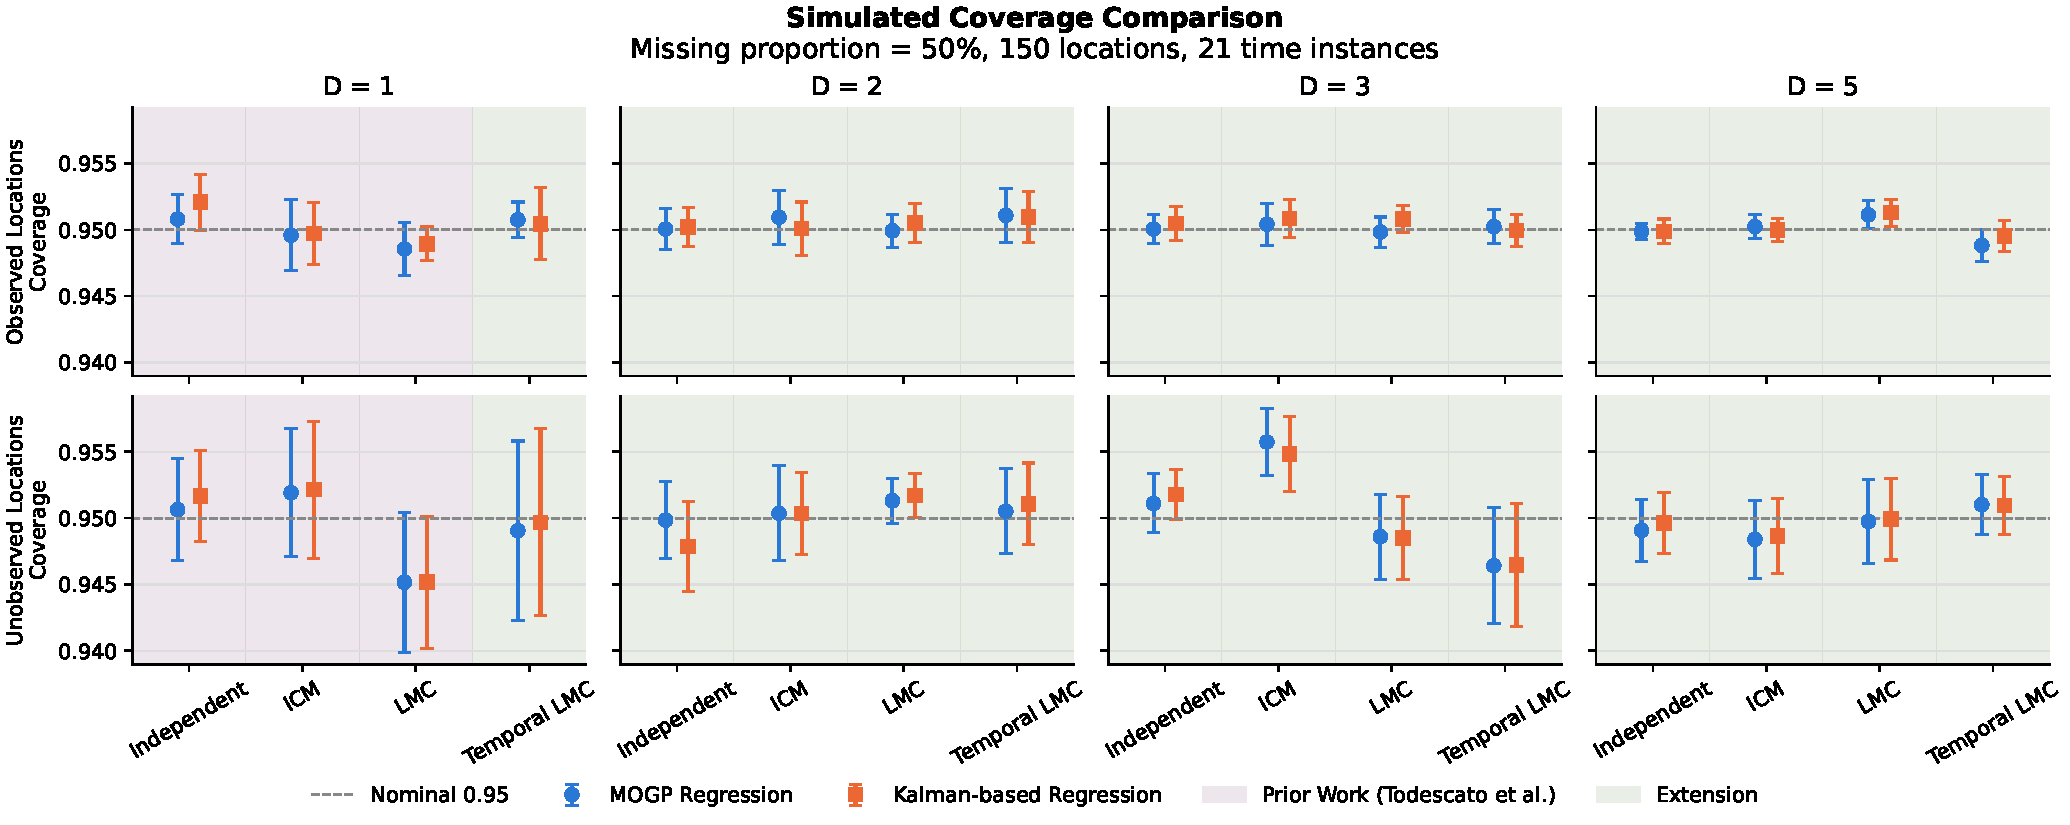
\includegraphics[height=0.35\textheight]{shaded_plots/coverage_missing_frac=0.5.pdf}

%         \caption{{\small Plots of empirical 95\% credible interval coverage for $\rho = 0\%$ (top) and $\rho = 50\%$ (bottom)}}
%     \end{figure}
% \end{frame}

\section{Discussion}
\begin{frame}{Conclusions}
    \begin{itemize}
        \item
        This project extends the Kalman-based Gaussian process regression algorithm of \citet{Todescato-Efficient-2020} for multi-output spatiotemporal dynamical systems. 
        \item 
        The multi-output method seems robust to some relaxation of the spatiotemporal kernel separability assumptions.
        \item
        Empirical accuracy in simulations is close to that of MOGP regression, and credible intervals are well-calibrated.
        \item 
        Most importantly, the Kalman-based MOGP regression method significantly increases the speed of computing predictions of the unknown states.
    \end{itemize}
\end{frame}

\begin{frame}{Limitations}
    \begin{itemize}
        \item
        The simulation study covers a limited number of combinations of settings, and could benefit from further extensions, such as alternative kernel functions and more complex state spaces. 
        \item 
        Computational and memory limits prevented simulations with $D > 5$, which are settings where our algorithm should most significantly outperform standard MOGP regression.
        \item
        The simulation study assumes that the kernel function $\bfK$ is known, which is a strict and unrealistic assumption.
    \end{itemize}
\end{frame}

\begin{frame}{Future Work}
    \begin{itemize}
        \item 
        \textbf{Real Data:} Apply the proposed multi-output algorithm to spatiotemporal datasets to assess how well the modelling assumptions hold in practice. 
        \item 
        \textbf{Unknown Dynamics:} Learn kernel hyperparameters jointly with latent states in the model using methods such as variational inference or empirical Bayes.
        \item \textbf{Change-points:} Extend the algorithm to dynamical systems whose underlying mechanics change at some point in time.
    \end{itemize}
\end{frame}

\begin{frame}[allowframebreaks]{References}
    \footnotesize
    \nocite{Sarkka-GP-KF-2013,Bayesian-Filter-Book-2023}
    \bibliography{presentation-references}
\end{frame}

\appendix

% \section{Plots}

\section{Algorithms}

\begin{frame}{Kalman Filtering Algorithm \citep{Kalman-Filter-1960}}
    \footnotesize
    \begin{algorithmic}[1]
        \Require
            \Statex \hspace{\algorithmicindent} $\widehat{\bfm}(0 \mid 0)$: expected value of the initial state $\bfs(0)$       
            \Statex \hspace{\algorithmicindent} $\bfSigma(0 \mid 0)$: variance of the initial latent state $\bfs(0)$
        \For{$j = 1$ to $J$}
            \Statex \texttt{\# Prediction Step:}
            \State $\widehat{\bfm}(j \mid j-1) = \bfA(j-1)\widehat{\bfm}(j-1 \mid j-1)$
            \State $\bfSigma(j \mid j-1) = \bfA(j-1)\bfSigma(j-1 \mid j-1)\bfA(j-1)^{\sfTsmall} + \bfQ(j-1)$

            \Statex \texttt{\# Update Step:}
            \State $\bfd(j) = \bfy(j) - \bfC(j)\widehat{\bfm}(j \mid j-1)$
            \State $\bfS(j) = \bfC(j)\bfSigma(j \mid j-1)\bfC(j)^{\sfTsmall} + \bfR(j)$
            \State $\bfK(j) = \bfSigma(j \mid j-1)\bfC(j)^{\sfTsmall}\bfS(j)^{-1}$ % \Comment{Kalman gain}
            \State $\widehat{\bfm}(j \mid j) = \widehat{\bfm}(j \mid j-1) + \bfK(j)\bfd(j)$
            \State $\bfSigma(j \mid j) = \bfSigma(j \mid j-1) - \bfK(j)\bfS(j)\bfK(j)^{\sfTsmall}$
        \EndFor
    \end{algorithmic}
\end{frame}

\begin{frame}{Kalman-Enhanced GP Regression \citep{Todescato-Efficient-2020}}
    \footnotesize
    \begin{algorithmic}[1]
        \Require $(F,G,H)$, $\sigma^{2}$, $\calI$, $K_{s}$, $\gamma$, $\bfSigma_{0}$
        \State $\widehat{\bfs}(0 \mid 0) = \mathbf{0}$, $\bfSigma(0 \mid 0) = \bfI \otimes \bfSigma_{0}$, $j \gets 0$
        \Statex \texttt{\# Kalman updates}
        \While{$j \le J$ and $t_{j+1} \le t$}
            \State Compute $A(j), C(j), Q(j), R(j)$
            \State Compute $\widehat{\bfs}(j+1 \mid j+1), \bfSigma(j+1 \mid j+1)$ via Kalman filter update
            \State $j \gets j + 1$
        \EndWhile
        \Statex \texttt{\# Open-loop prediction}
        \State $\tau = t - t_{j}$
        \State $\widehat{\bfs}(t) = \big(e^{\tau(\bfI \otimes F)}\big)\,\widehat{\bfs}(j \mid j)$
        \State $\bfSigma^{\bfs}(t) = \big(e^{\tau(\bfI \otimes F)}\big)\bfSigma(j \mid j)\big(e^{\tau(\bfI \otimes F)}\big)^{\sfTsmall}$
        \Statex \texttt{\# Process estimate}
        \State $\widehat{\bff}(t) = \overline{K}_{s}^{1/2}(\bfI \otimes H)\,\widehat{\bfs}(t)$
        \State $\bfSigma^{\bff}(t) = \overline{K}_{s}^{1/2}(\bfI \otimes H)\bfSigma^{\bfs}(t)(\bfI \otimes H)^{\sfTsmall}\,\overline{K}_{s}^{1/2}$
        \State \Return $\widehat{\bff}(t)$, $\bfSigma^{\bff}(t)$
    \end{algorithmic}    
\end{frame}

\begin{frame}{Kalman-Enhanced MOGP Regression (Hotz, 2026)}
    \footnotesize
    \begin{algorithmic}[1]
        \Require $\{(F_{q},G_{q},H_{q})\}_{q=1}^{Q}$, $\bfV$, $\calI$, $\{K_{s}^{(q)}\}_{q=1}^{Q}$, $\{\bfB^{(q)}\}_{q=1}^{Q}$, $\{\gamma^{(q)}\}_{q=1}^{Q}$, $\bfSigma_{0}$
        \State Build companion matrices $\overline{F}, \overline{G}, \{\widetilde{H}_{q}\}_{q=1}^{Q}$
        \State $\bfH = \sum_{q=1}^{Q}\big([\overline{K}_{s}^{(q)}]^{1/2} \otimes [\bfB^{(q)}]^{1/2}\big)(\bfI_{MD} \otimes \widetilde{H}_{q})$
        \State $\widehat{\bfs}(0 \mid 0) = \mathbf{0}$, $\bfSigma(0 \mid 0) = \bfI_{MD} \otimes \bfSigma_{0}$, $j \gets 0$
        \Statex \texttt{\# Kalman updates}
        \While{$j \le J$ and $t_{j+1} \le t$}
            \State Compute $A(j), C(j), Q(j), R(j)$
            \State Compute $\widehat{\bfs}(j+1 \mid j+1), \bfSigma(j+1 \mid j+1)$ via Kalman filter update
            \State $j \gets j + 1$
        \EndWhile
        \Statex \texttt{\# Open-loop prediction}
        \State $\tau = t - t_{j}$
        \State $\widehat{\bfs}(t) = \big(e^{\tau(\bfI \otimes \overline{F})}\big)\,\widehat{\bfs}(j \mid j)$
        \State $\bfSigma^{\bfs}(t) = \big(e^{\tau(\bfI \otimes \overline{F})}\big)\bfSigma(j \mid j)\big(e^{\tau(\bfI \otimes \overline{F})}\big)^{\sfTsmall}$
        \Statex \texttt{\# Process estimate}
        % \State $\widehat{\bff}(t) = \overline{K}_{s}^{1/2}(\bfI \otimes H)\,\widehat{\bfs}(t)$
        \State $\widehat{\bff}(t) = \bfH\,\widehat{\bfs}(t)$
        % \State $\bfSigma^{\bff}(t) = \overline{K}_{s}^{1/2}(\bfI \otimes H)\bfSigma^{\bfs}(t)(\bfI \otimes H)^{\sfTsmall}\,\overline{K}_{s}^{1/2}$
        \State $\bfSigma^{\bff}(t) = \bfH\,\bfSigma^{\bfs}(t)\,\bfH^{\sfTsmall}$
        \State \Return $\widehat{\bff}(t)$, $\bfSigma^{\bff}(t)$
    \end{algorithmic}   
\end{frame}

\section{Definitions}

\begin{frame}{Power Spectral Density}  
    \begin{definitionblock}{Power Spectral Density}
        The power spectral density (PSD) of a univariate real-valued function $z(\tau)$ is
        \begin{equation*}
            S(\omega) = \int z(\tau)e^{-2\pi{i}\omega\tau}\dx[\tau]
        \end{equation*}        
    \end{definitionblock} 
\end{frame}

\begin{frame}{Stationary and Isotropic Kernels}
    \begin{definitionblock}{Stationary Kernel}
        A kernel function $k: \calX \times \calX \to \bbR$ is a stationary kernel if the function can be written in the form $k(x, x') = \varphi(x - x')$ for some $\varphi: \bbR \to \bbR$. 
    \end{definitionblock}

    \begin{definitionblock}{Isotropic Kernel}
        A kernel function $k: \calX \times \calX \to \bbR$ is isotropic if it can be written in the form $k(x, x') = \kappa(\norm{x - x'})$ for some $\kappa: \bbR \to \bbR$.
    \end{definitionblock}
\end{frame}

\begin{frame}{RBF and Mat{\'e}rn Kernels}
    \begin{itemize}
        \item     
        The RBF and Mat{\'e}rn kernels are standard isotropic kernel functions often used in Gaussian process regression.
        \item 
        For these functions, we set $d := \norm{x - x'}$, with scaling hyperparameters $\sigma^{2}$ and $\ell$. 
    \end{itemize}
    {\small
    \begin{align*}
        \textnormal{\textbf{Mat{\'e}rn(1/2):}} &\quad C_{1/2}(x, x') = \sigma^{2}\exp\!\Big(-\frac{d}{\ell}\Big)\\
        \textnormal{\textbf{Mat{\'e}rn(3/2):}} &\quad C_{3/2}(x, x') = \sigma^{2}\Big(1 + \frac{\sqrt{3}d}{\ell}\Big)\exp\!\Big(-\frac{\sqrt{3}d}{\ell}\Big)\\
        \textnormal{\textbf{Mat{\'e}rn(5/2):}} &\quad C_{5/2}(x, x') = \sigma^{2}\Big(1 + \frac{\sqrt{5}d}{\ell} + \frac{{5}d^{2}}{3\ell^{2}}\Big)\exp\!\Big(-\frac{\sqrt{5}d}{\ell}\Big)\\
        \textnormal{\textbf{Gaussian (RBF):}} &\quad K_{\textrm{RBF}}(x, x') = \sigma^{2}\exp\!\Big(-\frac{d^{2}}{2\ell^{2}}\Big)
    \end{align*}  
    }  
\end{frame}

% \section{Theoretical Results}

% \begin{frame}{Proof of Dynamic Representer Theorem}
%     \begin{itemize}
%         \item 
%     \end{itemize}
% \end{frame}

% \begin{frame}{Gaussian Process Complexity}
%     \begin{itemize}
%         \item GP regression on a dataset containing $N$ observations typically has a $\calO(N^{3})$ computational cost. 
%         \item The computational bottleneck arises from computing the \emph{Cholesky factorization} $\bfK = \bfL\bfL^{\sfTsmall}$ \citep{GPML-Book-2006}.
%     \end{itemize}   
% \end{frame}

% \begin{frame}{Kalman Filter Complexity}
%     \begin{itemize}
%         \item 
%     \end{itemize}
% \end{frame}

% \begin{frame}{State-Space Representation}
%     \begin{itemize}
%         \item The state-space representation $(F, G, H)$
%     \end{itemize}
% \end{frame}

\section{Plots}

\begin{frame}[allowframebreaks]{Results: RMSE}
    \centering
    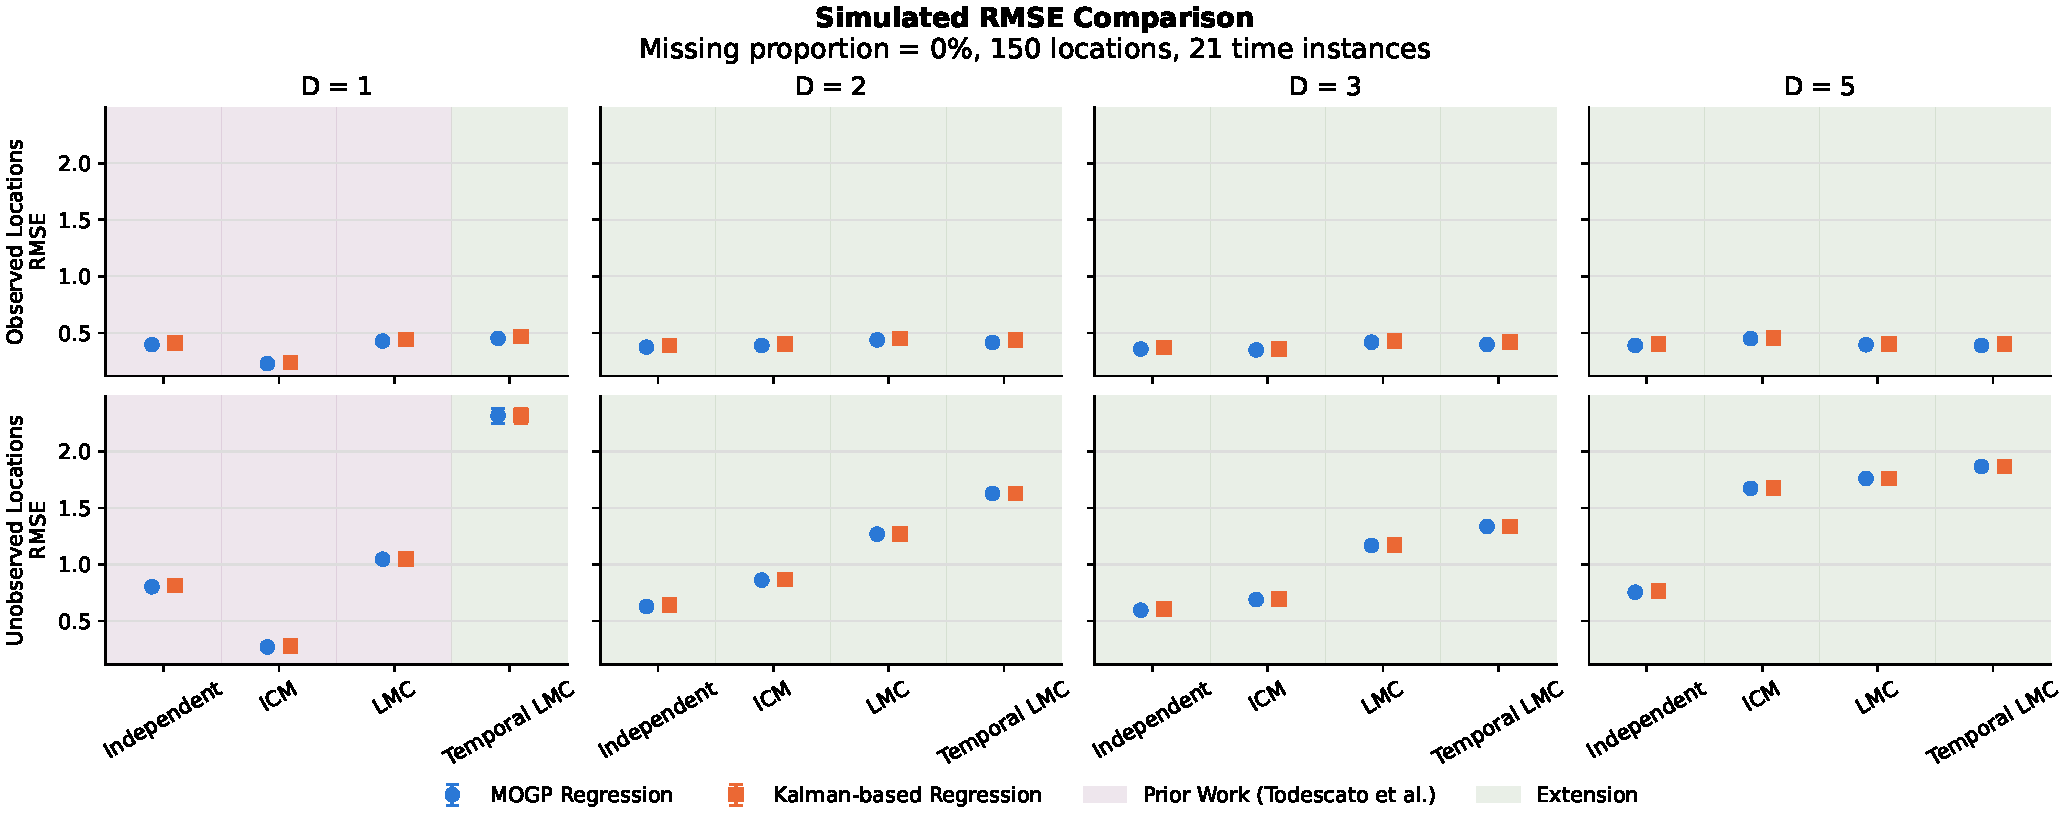
\includegraphics[width=0.95\textwidth]{shaded_plots/rmse_missing_frac=0.0.pdf}\\[1em]
    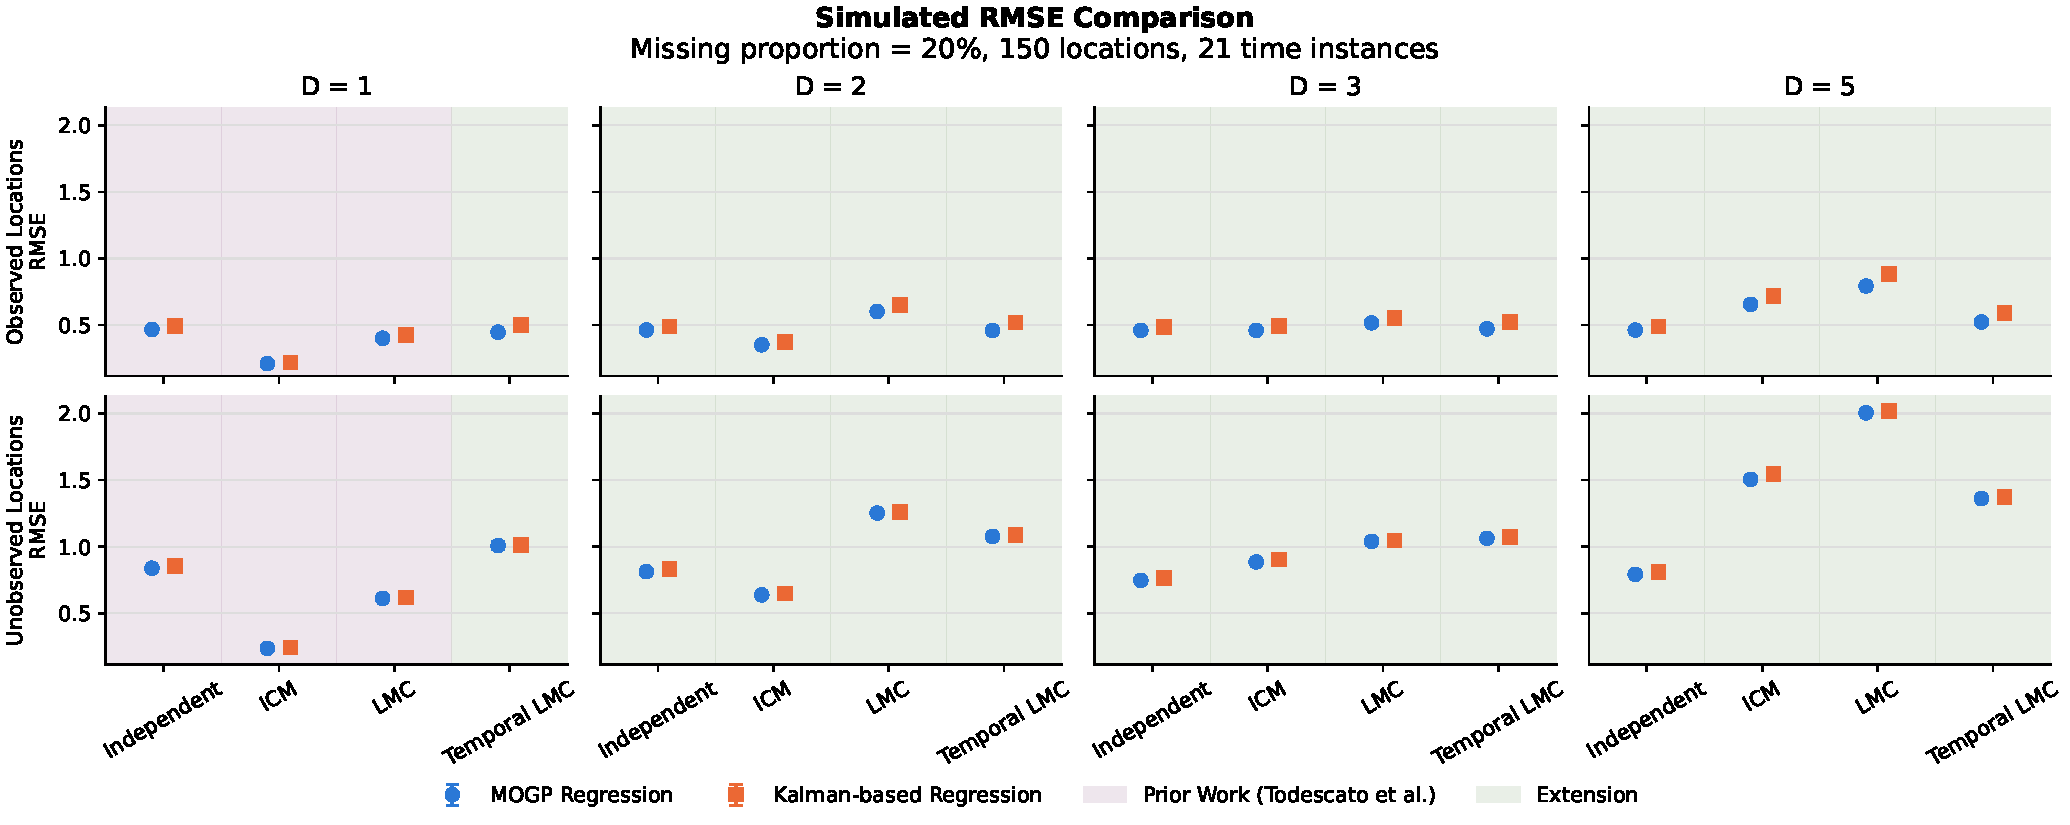
\includegraphics[width=0.95\textwidth]{shaded_plots/rmse_missing_frac=0.2.pdf}\\[1em]
    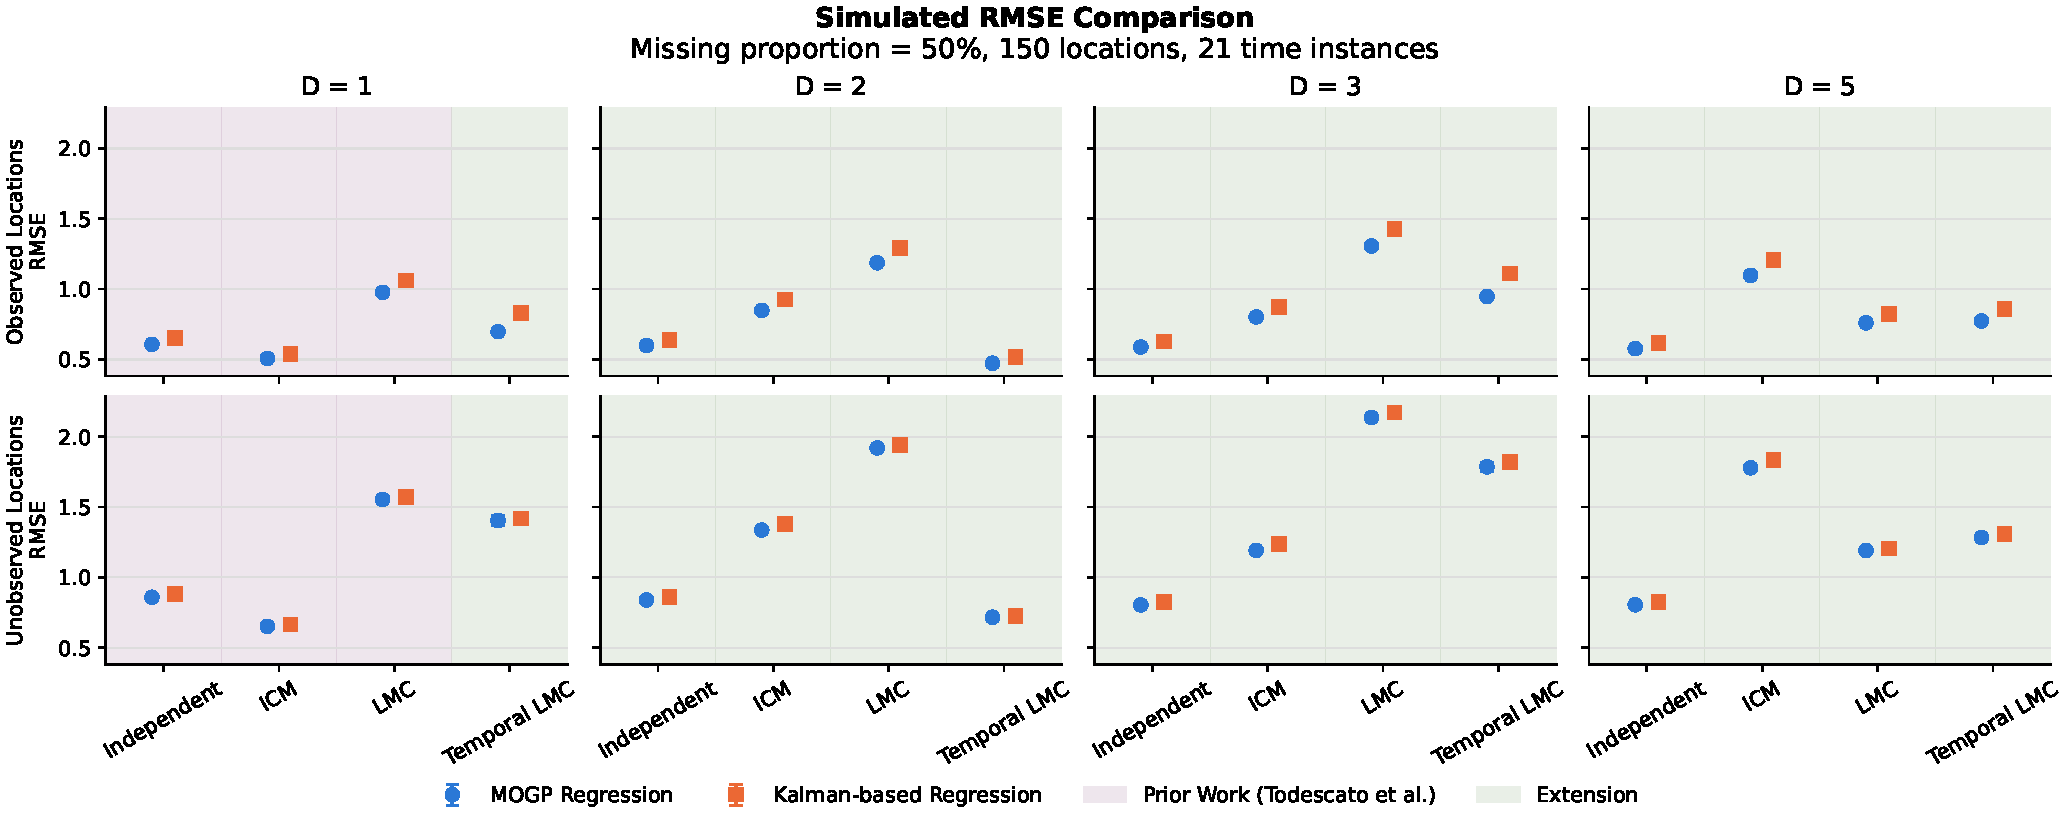
\includegraphics[width=0.95\textwidth]{shaded_plots/rmse_missing_frac=0.5.pdf}
\end{frame}

\begin{frame}[allowframebreaks]{Results: Wall Clock Time}
    \centering
    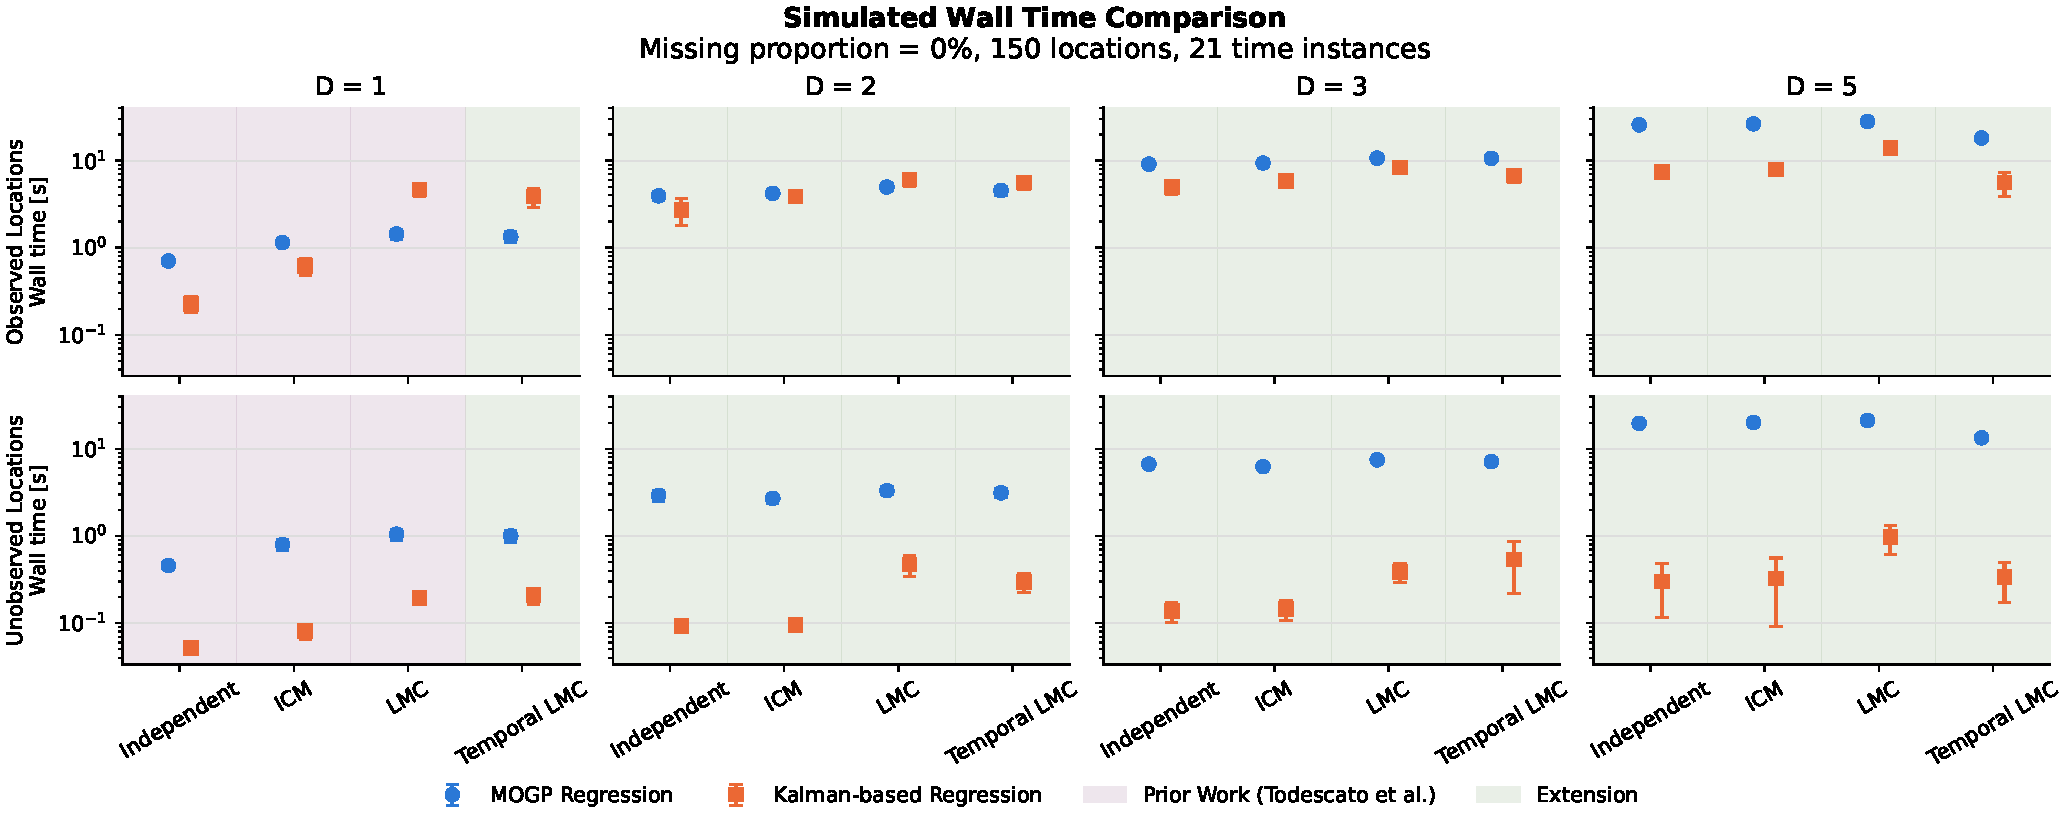
\includegraphics[width=0.95\textwidth]{shaded_plots/wall_time_missing_frac=0.0.pdf}\\[1em]
    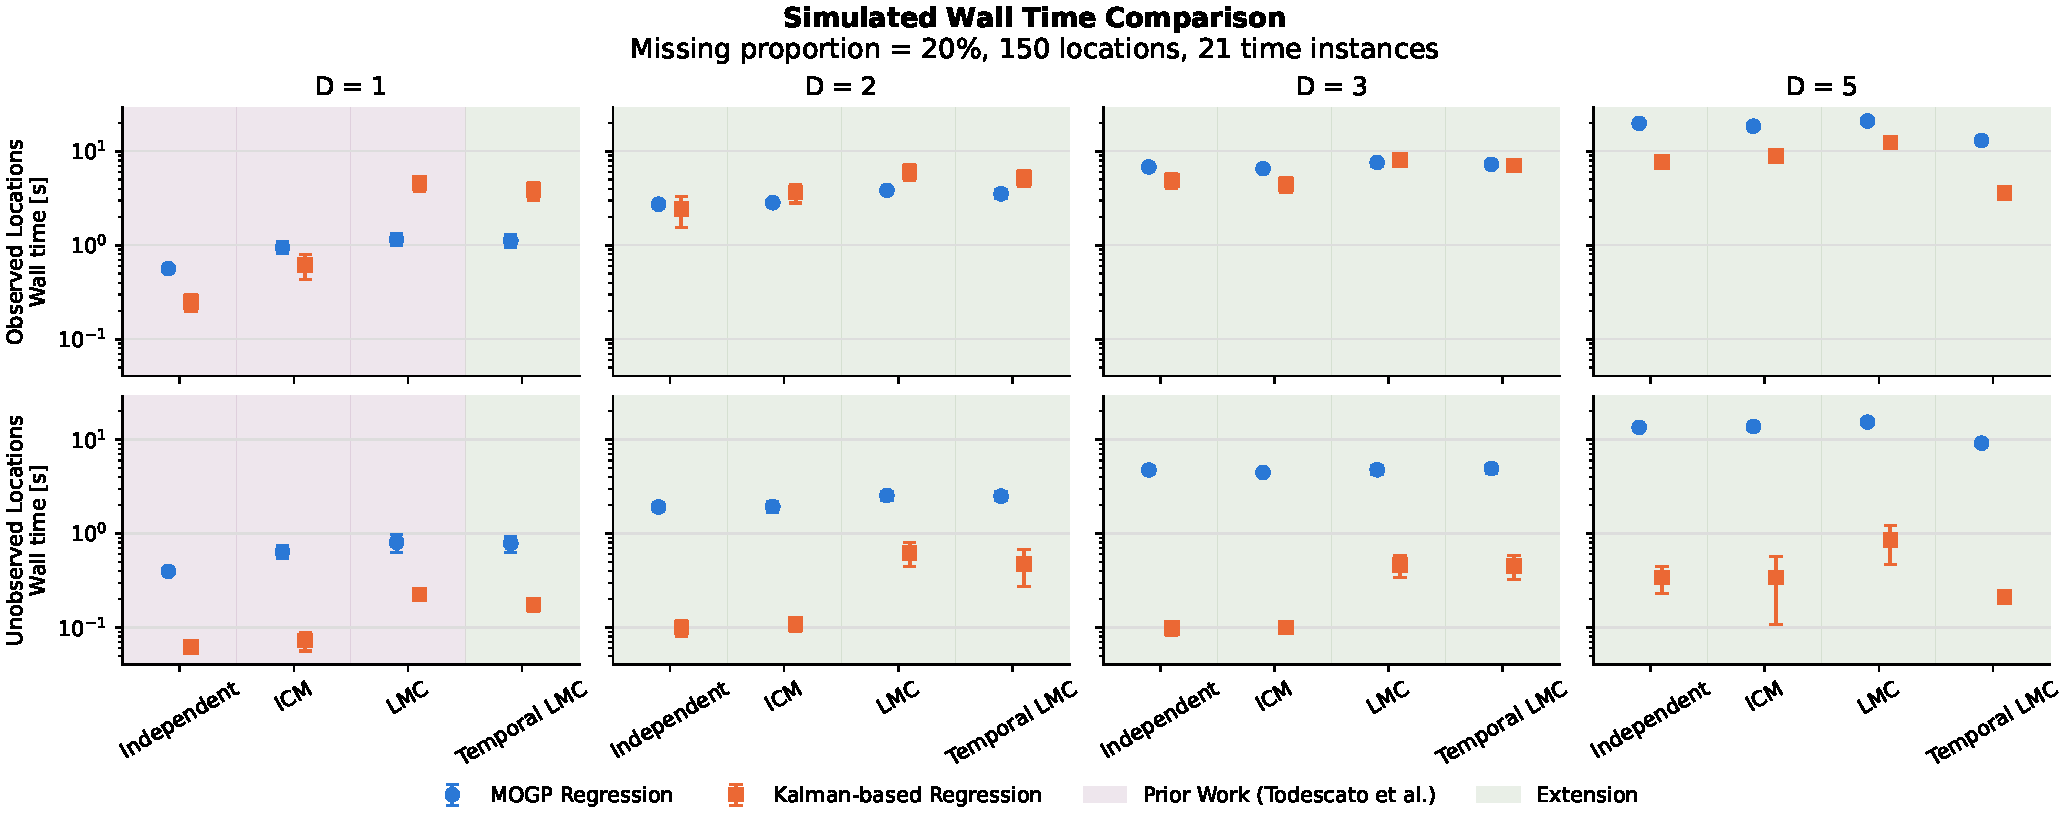
\includegraphics[width=0.95\textwidth]{shaded_plots/wall_time_missing_frac=0.2.pdf}\\[1em]
    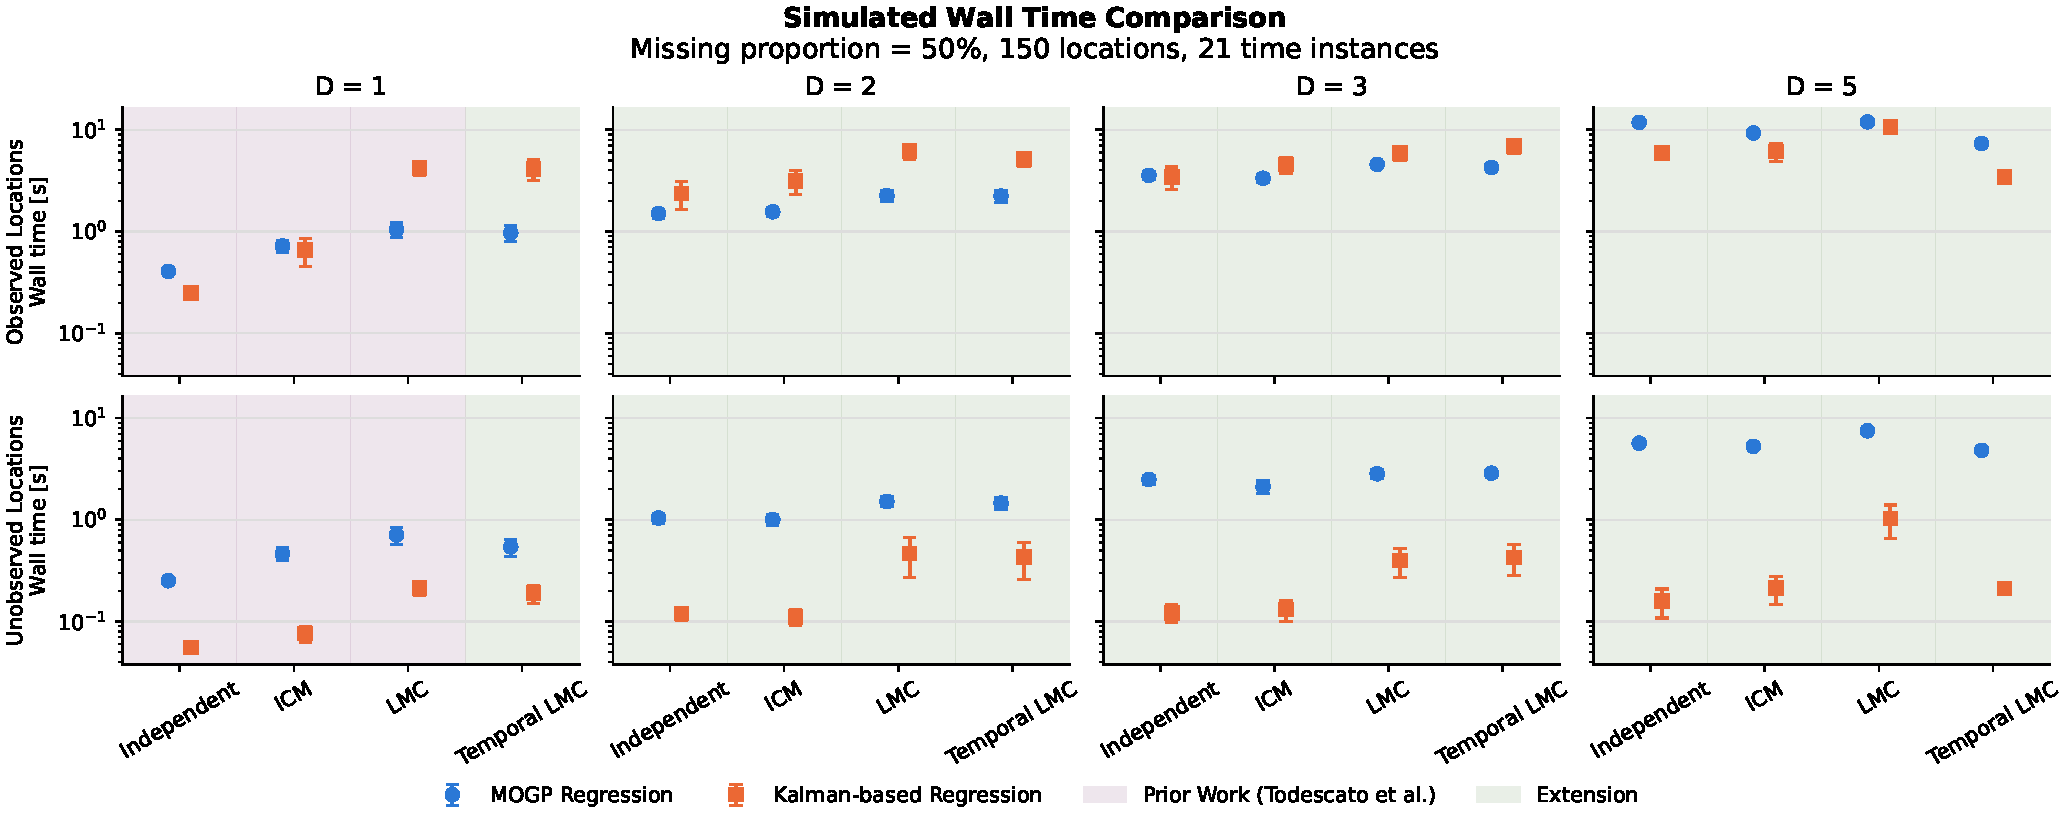
\includegraphics[width=0.95\textwidth]{shaded_plots/wall_time_missing_frac=0.5.pdf}
\end{frame}

\begin{frame}[allowframebreaks]{Results: MAE}
    \centering
    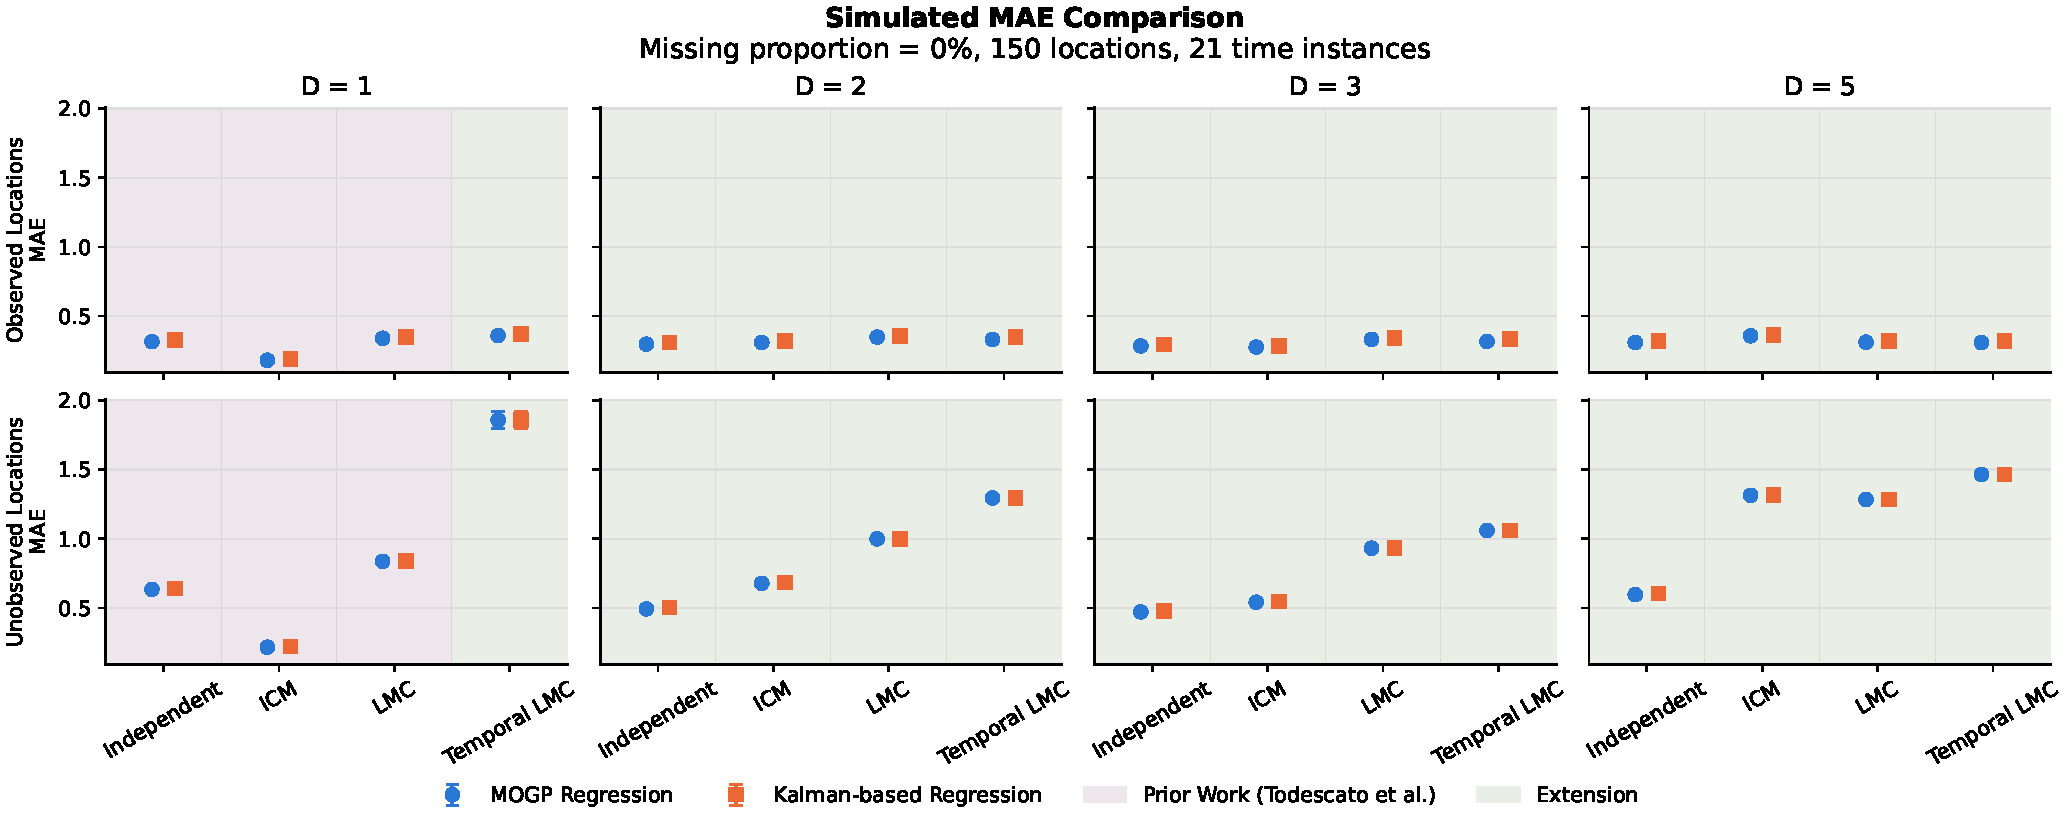
\includegraphics[width=0.95\textwidth]{shaded_plots/mae_missing_frac=0.0.pdf}\\[1em]
    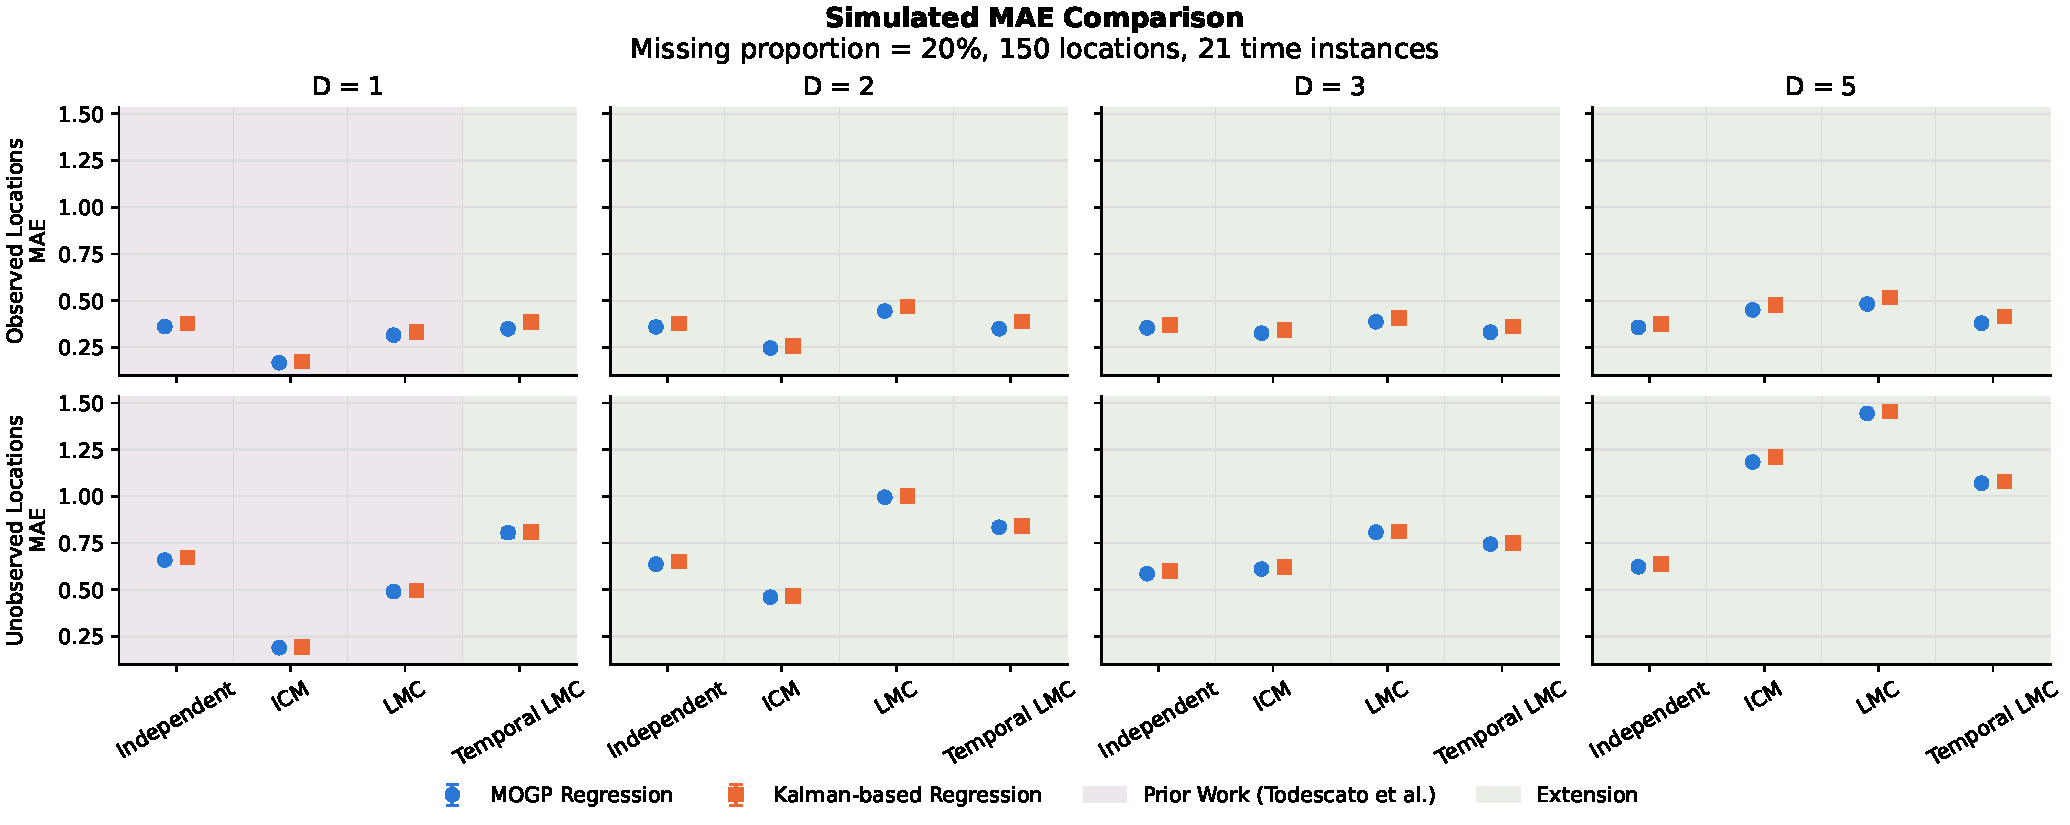
\includegraphics[width=0.95\textwidth]{shaded_plots/mae_missing_frac=0.2.pdf}\\[1em]
    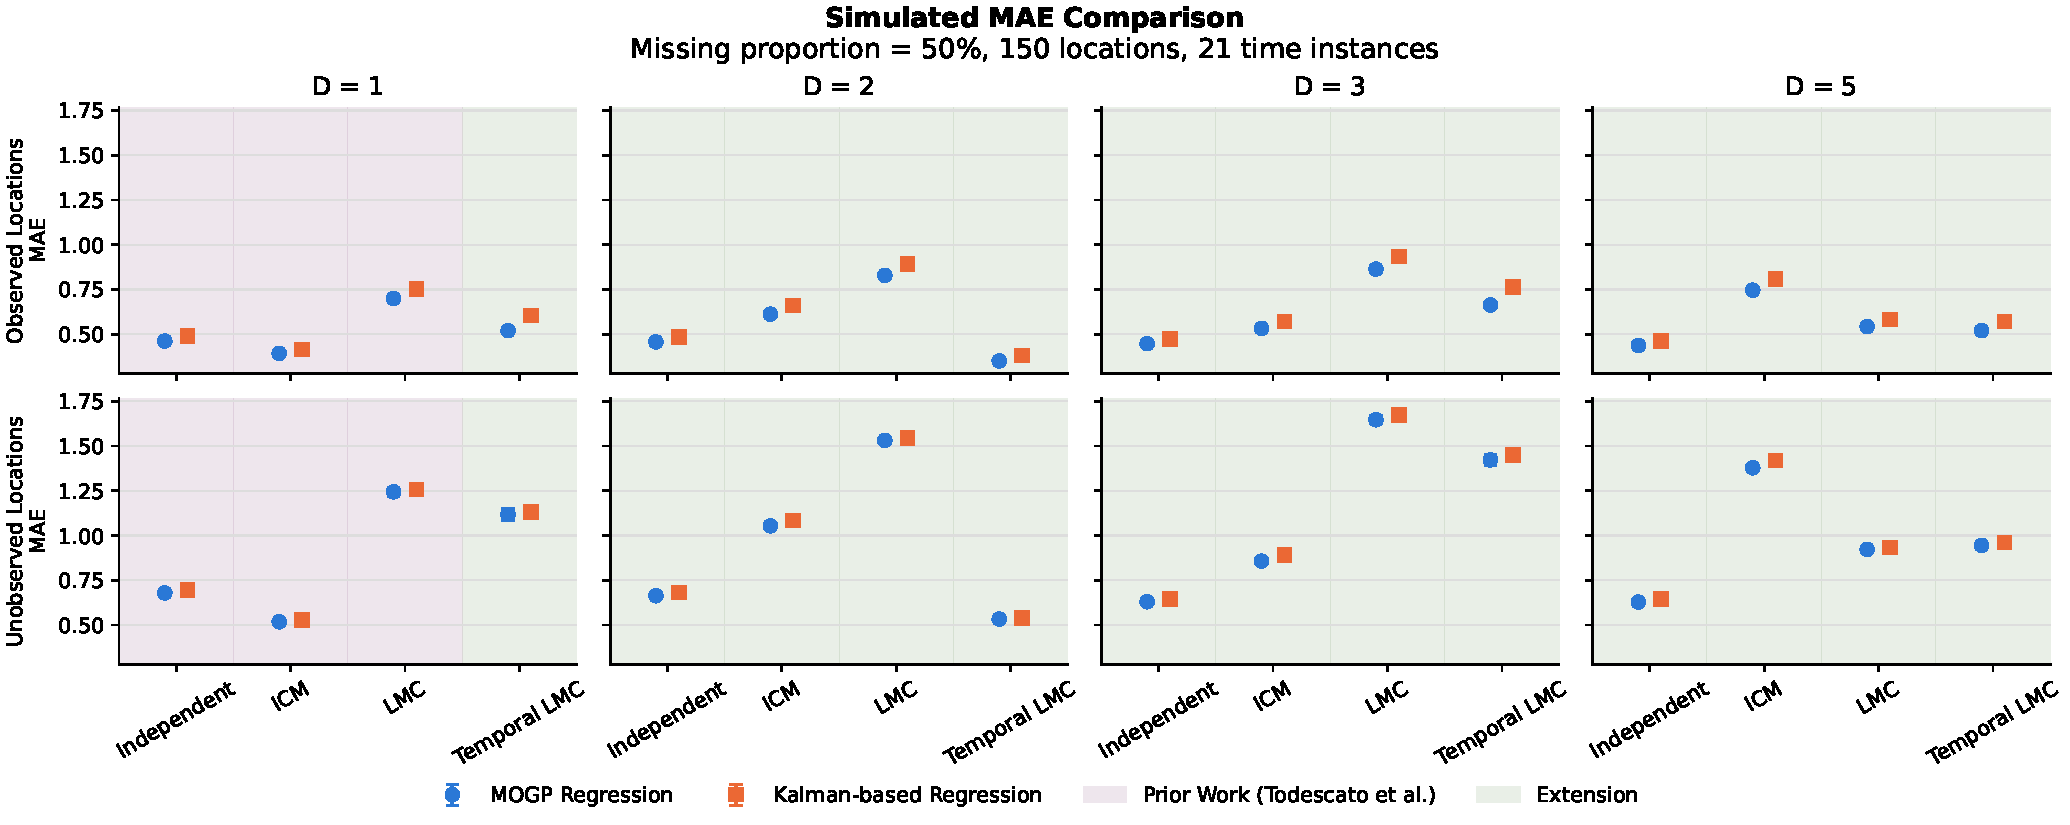
\includegraphics[width=0.95\textwidth]{shaded_plots/mae_missing_frac=0.5.pdf}
\end{frame}

\begin{frame}[allowframebreaks]{Results: Coverage}
    \centering
    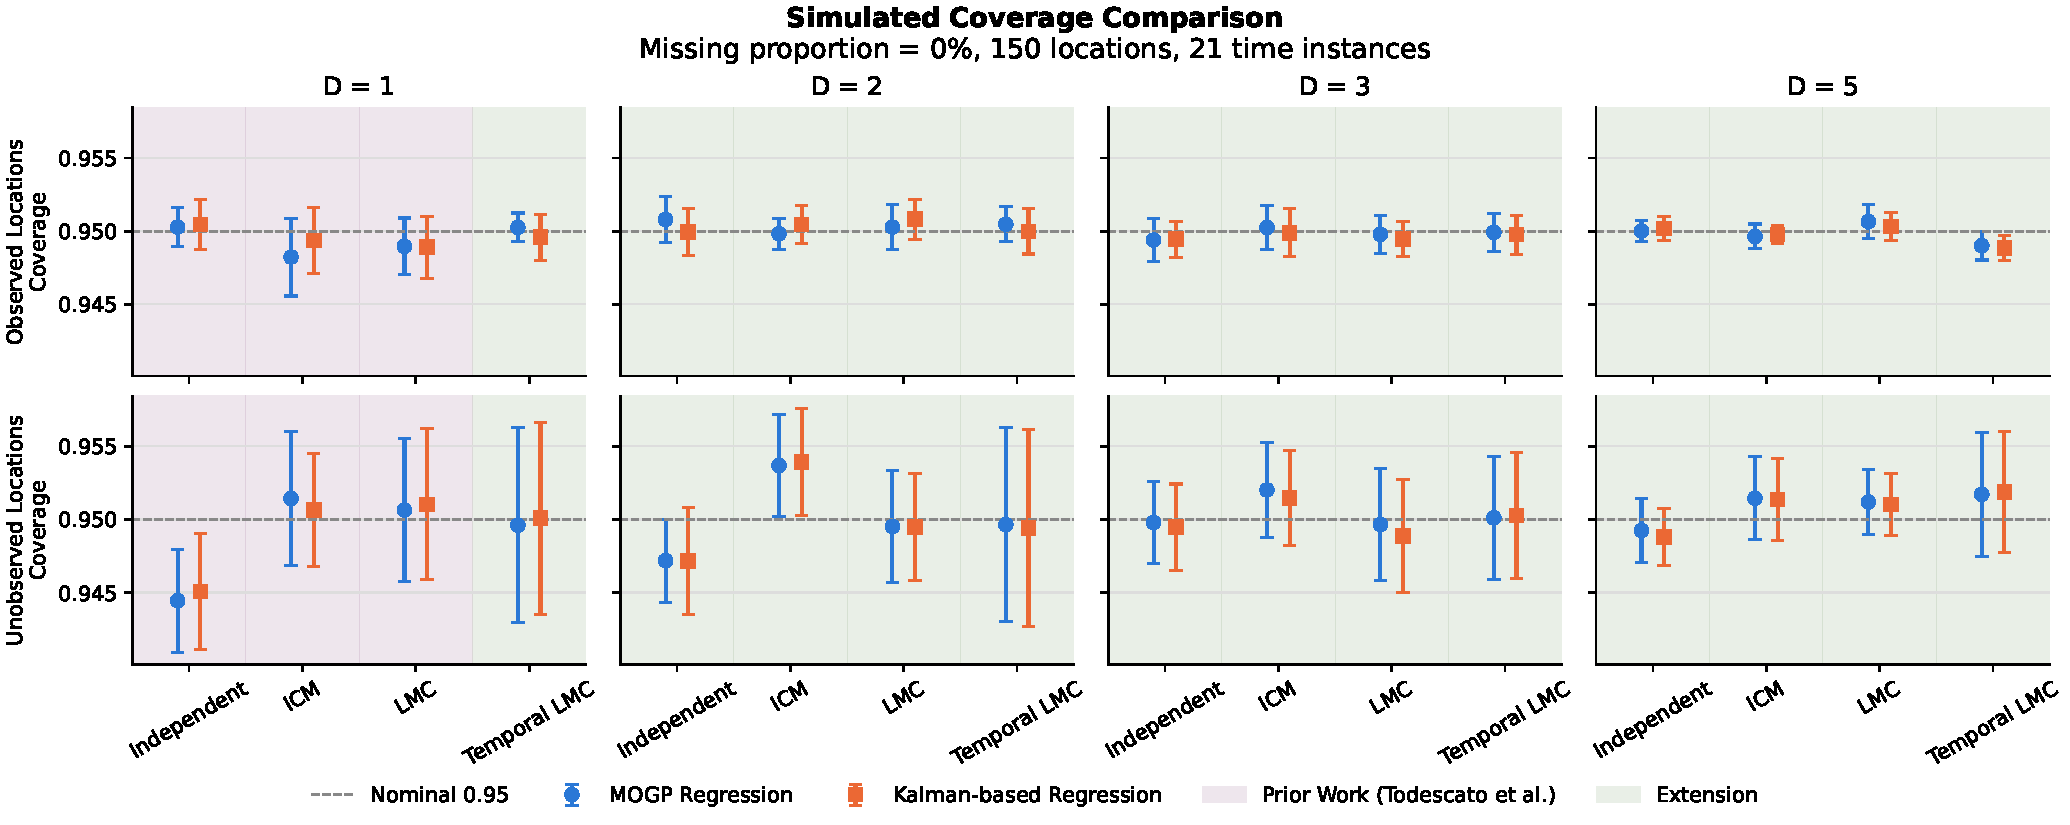
\includegraphics[width=0.95\textwidth]{shaded_plots/coverage_missing_frac=0.0.pdf}\\[1em]
    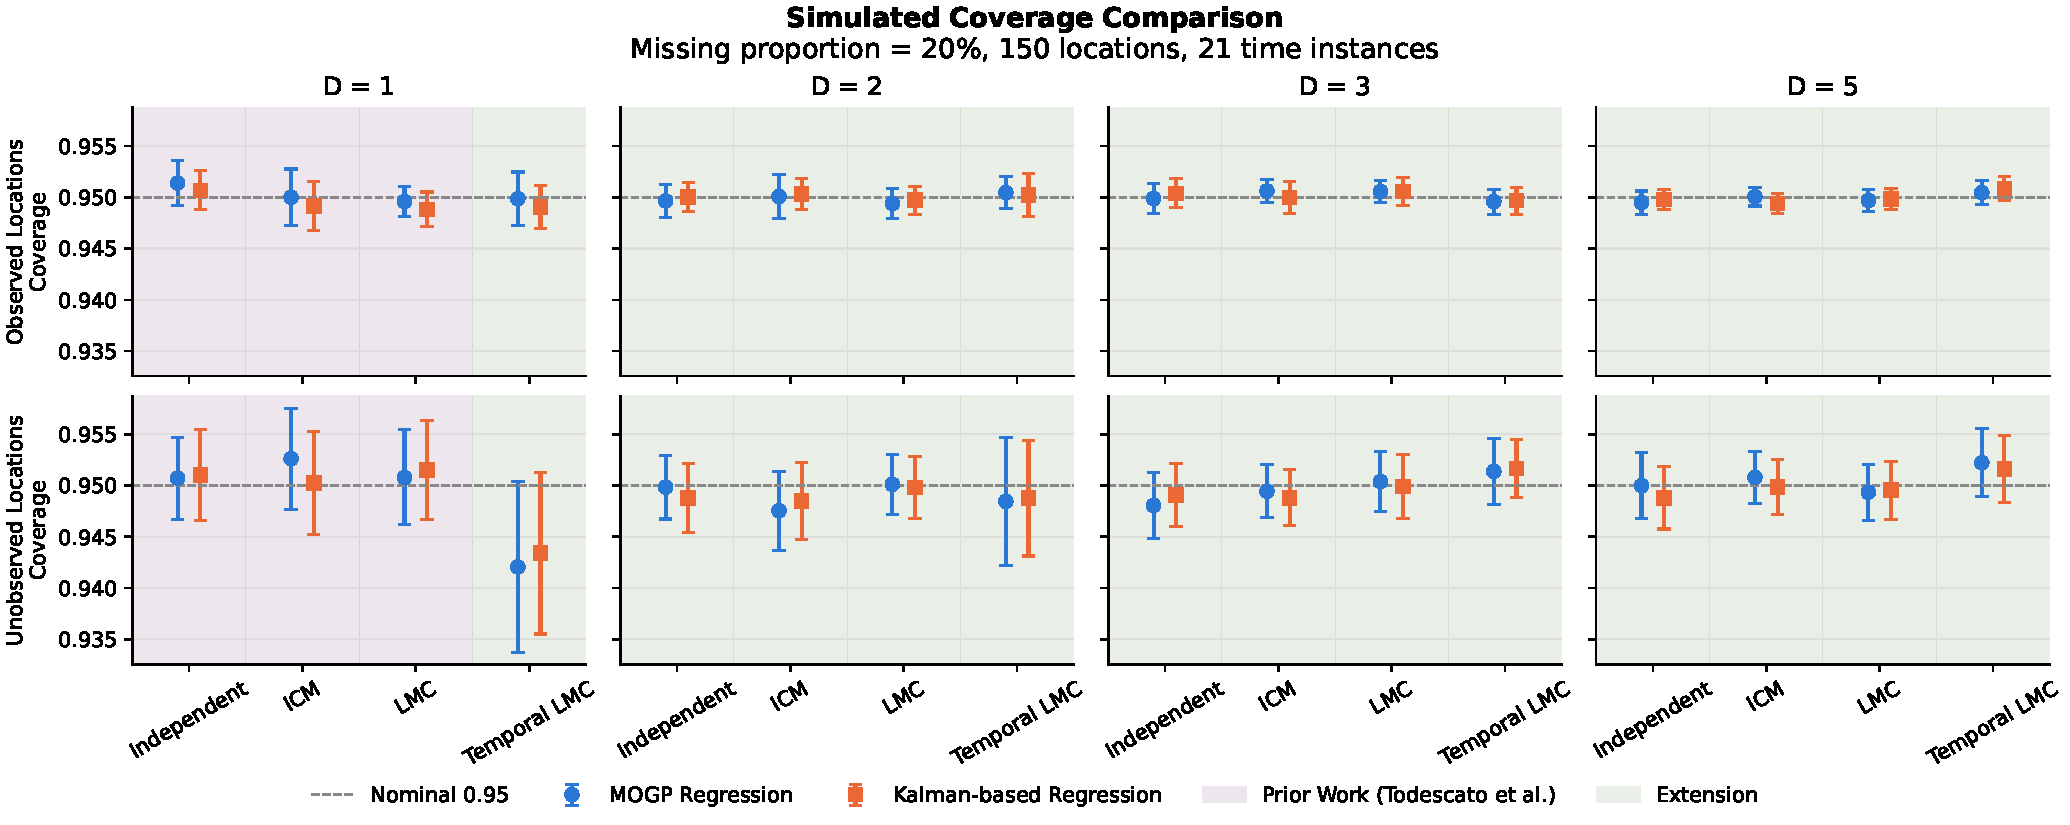
\includegraphics[width=0.95\textwidth]{shaded_plots/coverage_missing_frac=0.2.pdf}\\[1em]
    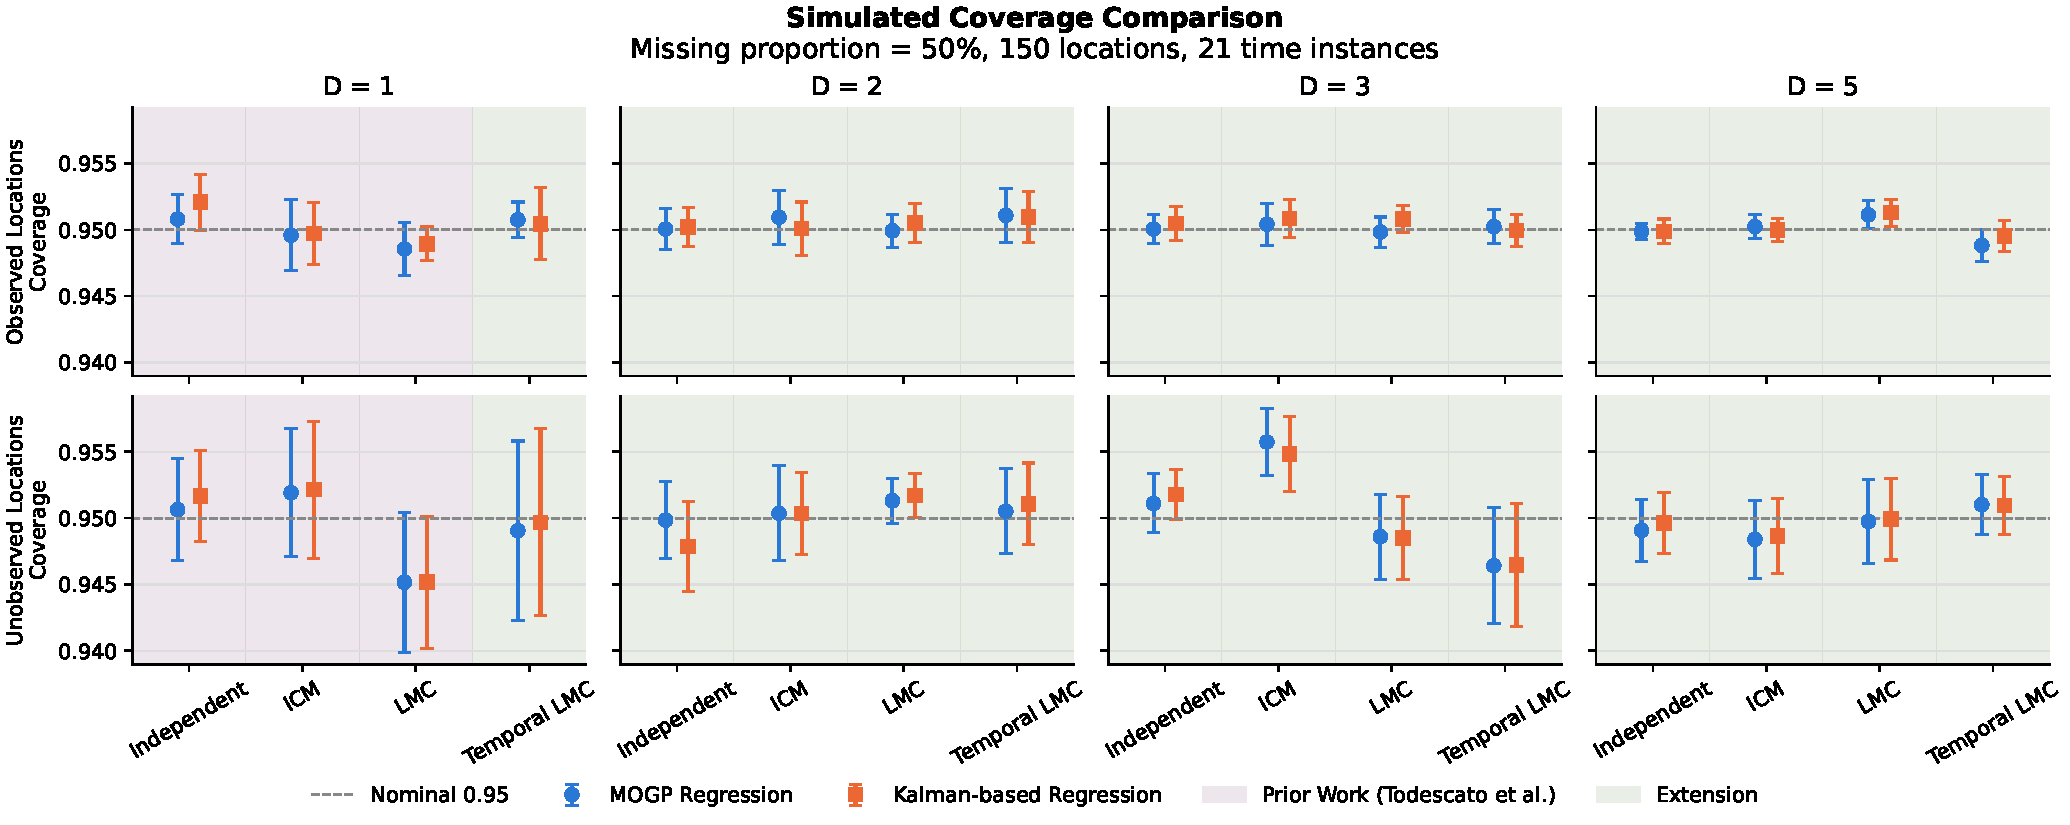
\includegraphics[width=0.95\textwidth]{shaded_plots/coverage_missing_frac=0.5.pdf}
\end{frame}

\end{document}
